\documentclass{ieeeaccess}
\usepackage{cite}
\usepackage{amsmath,amssymb,amsfonts}
\usepackage{graphicx}
\usepackage{textcomp}
\usepackage{booktabs}
\usepackage{array}
\usepackage{multirow}
\usepackage{algorithm}
\usepackage{algpseudocode}

\def\BibTeX{{\rm B\kern-.05em{\sc i\kern-.025em b}\kern-.08em
    T\kern-.1667em\lower.7ex\hbox{E}\kern-.125emX}}

\begin{document}
\history{}
\doi{}

\title{Event-Aware Virtual Power Plant Dispatch via Language-Enhanced Soft Actor-Critic Reinforcement Learning With a Semantic Safety Layer}

\author{\uppercase{Xingchen Li}\authorrefmark{1}, and \uppercase{Jijun Wang}\authorrefmark{2}}
\address[1]{Shanghai University of Electric Power, Shanghai, China (e-mail: to be added)}
\address[2]{Shanghai University of Electric Power, Shanghai, China (e-mail: to be added)}
\tfootnote{This work received no external funding.}

\markboth
{Li \headeretal: Event-Aware VPP Dispatch via Language-Enhanced SAC With a Semantic Safety Layer}
{Li \headeretal: Event-Aware VPP Dispatch via Language-Enhanced SAC With a Semantic Safety Layer}

\corresp{Corresponding author: Xingchen Li (e-mail: to be added).}

\begin{abstract}
Virtual power plants (VPPs) increasingly operate under renewable uncertainty, market-price volatility, and external events described in natural language, such as weather warnings, demand-response notices, and renewable-curtailment alerts. Most reinforcement-learning dispatch methods use only numerical states and therefore cannot directly exploit these signals. This paper proposes a language-enhanced Soft Actor-Critic framework (LE-DRL-SAC) for event-aware VPP battery dispatch. A large language model (DeepSeek) is used only as a semantic encoder: it converts operational text into structured risk features, which are fused with numerical VPP states and consumed by an SAC policy. The language model never emits dispatch actions. The learned action is further blended with a deterministic semantic safety layer whose weight is treated as event-coverage dependent. On a public-data-calibrated 15-minute VPP dispatch dataset with four event scenarios, LE-DRL-SAC with the semantic safety layer ($w=0.9$) achieves the best average total reward, outperforming numerical SAC, text-ablation SAC, a numeric-safety-layer ablation, rule-based control, enhanced rolling-horizon optimization, and Linear-MPC. A semantic-source ablation confirms that the SAC actor reads LLM-derived features from the augmented state (native outperforming zeroed-semantics by $+792$ yuan, 20/20 seed-scenario pairs favorable) and that the semantic content, not merely the input dimensionality, carries the value. On a frequency-reserve event whose category lies outside the deployed keyword table, the LLM encoder supplies a usable semantic vector with zero reconfiguration and the language-enhanced policy exceeds the keyword-encoder baseline by $+789$ yuan (95\% CI $[+743, +838]$, 5/5 seeds), illustrating that the LLM's value surfaces precisely outside the coverage a hand-crafted encoder was built for. A real-price validation on a three-week German DE-LU day-ahead series and Open-Meteo weather further corroborates the adaptation under genuine, heterogeneous negative prices (gap $+$6{,}035~EUR, 95\% CI $[+$5{,}415, $+$6{,}656]).
\end{abstract}

\begin{keywords}
Virtual power plant, deep reinforcement learning, Soft Actor-Critic, large language model, semantic enhancement, battery dispatch, demand response, renewable curtailment.
\end{keywords}

\titlepgskip=-15pt
\maketitle

\section{Introduction}
\label{sec:introduction}
\PARstart{V}{irtual} power plants (VPPs) aggregate distributed photovoltaics (PV), battery energy storage, flexible loads, electric vehicles, and other distributed energy resources into controllable portfolios that participate in electricity markets and demand response. As renewable penetration and market-oriented operation intensify, VPP dispatch is no longer governed solely by load, PV output, price, and state of charge (SOC); operators must also respond to external information such as weather warnings, market announcements, demand-response invitations, and renewable-curtailment notices. These signals frequently arrive as natural-language text before their effects are fully reflected in numerical time series.

Deep reinforcement learning (DRL) has been extensively investigated for energy management and power-system control owing to its capacity to learn sequential policies from interaction data \cite{b1,b2,b9}. For battery dispatch, continuous-action algorithms such as Soft Actor-Critic (SAC) are particularly appealing because they can directly emit charging and discharging power commands \cite{b3,b11,b12}. Nevertheless, the majority of DRL dispatch controllers consume only numerical states, and the neglect of operational text constrains event awareness—most notably during high-temperature load-pressure, price-spike, and renewable-curtailment intervals.

Large language models (LLMs) offer a promising interface between unstructured operational text and numerical decision models. Recent studies have examined LLMs for power-system reasoning, dispatch assistance, and broader energy-sector applications \cite{b4,b5,b6}. However, directly commissioning an LLM to emit final dispatch actions is risky for power-system operation, because VPP dispatch must satisfy battery limits, SOC dynamics, market settlement logic, and reproducibility requirements. A more tractable design employs the LLM as a semantic front end: it transforms event text into structured risk features, whereas a conventional controller or reinforcement-learning policy generates the final action.

This study investigates the aforementioned decoupled design for VPP battery dispatch. The language module emits risk scores rather than free-form dispatch commands. The SAC actor furnishes the learned control component, while a deterministic semantic safety layer maps high-confidence textual risk cues into bounded action corrections. This hybrid design is motivated by a practical observation: a purely learned actor tends to underutilize rare event signals, whereas a pre-designed rule or prior can be strong only within the event categories it explicitly covers. When a new event category appears outside that coverage, cached LLM-derived semantic features can make the event observable to the learning actor without allowing the language model to bypass physical feasibility checks. Related work is reviewed in detail in Section~\ref{sec:related}.

The main contributions are as follows:
\begin{enumerate}
  \item A language-enhanced SAC framework is proposed for event-aware VPP battery dispatch. Operational text is converted into structured semantic risk features by an LLM-compatible semantic encoder and fused with numerical VPP states. The LLM serves as an advisor that emits risk scores rather than dispatch actions, and the SAC actor is the learned decision component.
  \item A semantic auxiliary reward and a semantic safety layer are introduced. The safety layer blends the learned actor action with a bounded risk-consistent prior, while all final actions remain subject to battery feasibility checks. The blending weight is treated as event-coverage-dependent rather than a universal constant, reflecting the observation that a pre-designed prior dominates on the event categories it was built for but must yield to a learning actor when the event falls outside its coverage.
  \item A new-event adaptation study is reported. A fifth event category---negative-price deep surplus---is absent from the hand-crafted prior and from the initial S1--S4 training set. During adaptation, the LLM semantic encoder is queried once for this new event to obtain cached risk scores, and the actor is retrained on S1--S5 while the prior is left unchanged. The study shows that when the semantic regularizer is relaxed, the language-enhanced policy exceeds numerical SAC on this new category (mean reward gap +5,482 yuan, 95\% bootstrap CI [+4,875, +6,074], all five seeds favorable), providing evidence that LLM-derived features help a reinforcement-learning dispatch policy adapt to an event category that the hand-crafted prior cannot cover. This is not a claim that an LLM directly outperforms a rule controller; rather, the LLM supplies structured event semantics that the SAC actor can exploit while the final action remains learned and feasibility-constrained. Crucially, this adaptation is not confined to the calibrated data: it is corroborated on a validation scenario built entirely from \emph{real} German DE-LU day-ahead prices (a three-week series, 2025-06-15 to 2025-07-05, with genuine inter-day heterogeneity) and \emph{real} Open-Meteo weather observations, where the language-enhanced policy retains a statistically significant advantage under genuine, heterogeneous negative prices (gap $+$6{,}035~EUR, 95\% CI $[+$5{,}415, $+$6{,}656], 5/5 seeds favorable). This real-price, real-weather result is the evidence closest to deployment and is the empirical anchor for the event-awareness claim in the title.
  \item A regularizer-sensitivity analysis reveals that the actor semantic-consistency regularizer, while stabilizing training on known events, suppresses the actor's adaptivity on the new negative-price event: lowering the regularizer weight improves the new-event reward by 18,515 yuan without degrading the four known-event scenarios. This finding refines the design of language-enhanced reinforcement-learning controllers by separating two roles of semantic information---a state feature that the actor can learn from, and a training target that constrains the actor.
  \item The calibrated VPP dataset is used for reproducible evaluation under four known event scenarios—normal summer operation, high-temperature load pressure, price spike, and renewable-curtailment pressure—and the method is compared with numerical SAC, a text-ablation SAC, a deterministic rule-based controller, a solver-free rolling-horizon optimizer, an engineering-regularized enhanced rolling-horizon optimizer, a Linear-MPC receding-horizon optimizer, a numeric-safety-layer SAC variant, random control, and Soft-Q baselines. The final configuration outperforms the implemented baselines in average total reward on the known-event scenarios.
  \item A semantic-source ablation isolates \emph{where} the language model contributes. Comparing three semantic sources (DeepSeek, a local keyword encoder, and noise-corrupted scores) against zeroed-semantics and numeric baselines shows that (i) the SAC actor genuinely reads the semantic state---native semantics beat zeroed semantics under the same input dimension by $+792$ yuan (20/20 seed-scenario pairs favorable) and corrupting the scores drops reward \emph{below} the zeroed baseline, so the semantic \emph{content}, not the input width, carries the value; (ii) on the four known categories the keyword encoder matches DeepSeek, so the LLM confers no distinct advantage where a hand-crafted table already covers the events; and (iii) on a frequency-reserve event outside that table the LLM encoder generalizes with zero reconfiguration while the keyword table returns all-zero scores, delineating the coverage boundary at which an LLM encoder becomes worthwhile rather than overclaiming universal superiority.
\end{enumerate}

\section{Related Work}
\label{sec:related}

\subsection{Optimization-Based VPP and Storage Dispatch}
Virtual power plants and battery storage dispatch have traditionally been formulated as mixed-integer linear programming (MILP), stochastic programming, or robust optimization problems that explicitly model forecast uncertainty, battery dynamics, and market settlement \cite{b10,b13,b14,b15}. Stochastic-programming offering models for VPP participation in electricity markets are reviewed in \cite{b10}, while model predictive control (MPC) has become a standard operational baseline for building and microgrid energy management \cite{b7,b16}. Although these optimization methods are interpretable and constraint-aware, they rely heavily on accurate forecasts and parameter tuning, and their online solving cost grows with horizon and state dimension. This paper keeps a rolling-horizon optimizer family as the optimization baseline, including an engineering-regularized enhanced variant. A Linear-MPC baseline (Scipy HiGHS LP solver, 24-step rolling horizon, terminal SOC penalty) is also implemented as a reference; its role is to anchor the comparison against a receding-horizon optimization that solves an explicit forecast-constrained LP at each step.

\subsection{Deep Reinforcement Learning for Energy Management}
DRL has been increasingly applied to energy storage arbitrage, microgrid management, and VPP dispatch. Actor-critic methods such as DDPG, TD3, and SAC are well suited to continuous charging/discharging control \cite{b3,b11,b12,b17,b18}, and comprehensive reviews summarize DRL applications across modern power and energy systems \cite{b9,b19,b20}. Relative to value-based discrete-action methods, maximum-entropy SAC offers a principled exploration--exploitation trade-off, which is particularly advantageous under price volatility and renewable uncertainty \cite{b3,b11}. A recurring limitation, however, is that most DRL dispatch controllers consume only numerical states and do not ingest textual operational signals. The present work targets this gap by augmenting the SAC state with language-derived risk features.

\subsection{Language Models and Semantic Information in Power Systems}
The recent LLM literature builds on the Transformer architecture \cite{b40}, scaling and few-shot behavior demonstrated by GPT-3-style models \cite{b41}, and the broader foundation-model paradigm in which a large pre-trained model is adapted to many downstream tasks while inheriting risks of opacity, bias, and failure propagation \cite{b42}. These properties explain both the attraction and the risk of using LLMs in power-system operation: they can parse heterogeneous operational language and domain instructions, but unconstrained text-generated actions are difficult to verify against physical and market constraints.

Recent surveys examine LLM capabilities and limitations in the electric energy sector. Majumder \emph{et al.}~\cite{b4} map the landscape of LLM use cases in electricity generation, transmission, and consumption, identifying knowledge retrieval, dispatch assistance, and text-driven decision support as promising directions while documenting hallucination and auditability risks that motivate keeping the LLM out of the final control loop. Amjad \emph{et al.}~\cite{b6}, Mirshekali \emph{et al.}~\cite{b36}, Zhang \emph{et al.}~\cite{b43}, and Yao \emph{et al.}~\cite{b44} provide complementary recent reviews of LLMs and large AI models for electrical power and energy systems, cataloguing applications in forecasting, operation support, fault diagnosis, energy management, document automation, perception, planning, and control, while emphasizing reproducibility, safety, computing cost, data privacy, and domain adaptation as barriers to deployment.

Beyond surveys, several studies have begun to instantiate LLMs in energy-system workflows. Cheng \emph{et al.}~\cite{b5} propose GAIA, an LLM for advanced power dispatch that uses language reasoning over operational contexts to support operation adjustment, monitoring, and black-start tasks. Huang \emph{et al.}~\cite{b37} discuss large foundation models for power systems and evaluate representative applications such as optimal power flow, electric-vehicle scheduling, knowledge retrieval, and situation awareness. Zhou \emph{et al.}~\cite{b38} introduce ElecBench, a power-grid-dispatch benchmark for evaluating LLMs across factuality, logicality, stability, security, fairness, and expressiveness, showing that domain-specific evaluation is necessary before operational deployment. For renewable forecasting, Wu and Ling~\cite{b53} propose STELLM, which adapts pre-trained language-model representations to spatio-temporal wind-speed forecasting. These works indicate that LLMs are moving from general question answering toward grid-specific reasoning, benchmarking, and time-series representation learning.

The adjacent building-energy and HVAC literature is especially relevant because it also combines text, operational data, and control or simulation workflows. Reviews by Zhang and Chen~\cite{b45} and Liu \emph{et al.}~\cite{b46} summarize LLM opportunities in building-energy applications, including energy management optimization, code generation, knowledge extraction, control support, and fault diagnosis. GPT-based studies have been used to automate data mining and pattern interpretation for building energy management and conservation \cite{b47}, to explain machine-learning control decisions under demand-response contexts \cite{b48}, to automate EnergyPlus-oriented building energy modeling and analysis \cite{b39,b49,b50,b51}, and to fine-tune domain-specific models for HVAC fault diagnosis \cite{b52}. These studies support the broader premise that operational text can be converted into structured engineering information, but most of them target modeling, diagnosis, forecasting, or decision support rather than closed-loop battery dispatch.

A common pattern across this literature is to deploy the language model as a feature extractor, advisor, interface, or evaluator rather than as the final controller, because directly LLM-generated actions are difficult to audit and constrain \cite{b4,b6,b38,b42}. The present work adheres to this pattern: the language module emits structured risk scores only, whereas a reproducible SAC actor and a deterministic safety layer generate the final action, so the LLM is queried once per event template and never participates in the per-step control loop. Relative to GAIA-style dispatch assistance, ElecBench-style LLM evaluation, building-energy modeling agents, and LLM-enhanced forecasting, this paper studies a narrower control question: whether cached LLM-derived event semantics can improve a reinforcement-learning battery-dispatch policy under known event categories and during adaptation to a newly introduced event category that a hand-crafted prior cannot cover.

\subsection{Safety Layers and Constrained Learning}
Deploying learned policies in safety-critical power-system settings necessitates constraint enforcement. Safe RL, constrained policy optimization, and action-shielding methods impose operational limits on top of learned actors \cite{b23,b24,b25,b26}. Action-prior blending and residual policy methods likewise combine a learned policy with a deterministic or rule-based base controller to guarantee feasibility \cite{b27,b28,b29}. Within the energy-management literature, hybrid schemes that couple rule-based or MPC supervisors with learned actors have been reported for microgrids and energy communities \cite{b8,b30,b31}. The present work is closest to the action-prior blending line: the semantic safety layer maps language-derived risk cues into a bounded correction blended with the SAC action, and the same blending formula is reused with a purely numeric prior to construct an ablation that isolates the value of textual semantics from the safety mechanism itself.

\subsection{Demand Response and Renewable-Curtailment Events}
Event-driven dispatch must additionally respond to demand-response invitations, weather warnings, and renewable-curtailment notices. Peer-to-peer energy systems, demand-response programs, and renewable-integration studies furnish the operational context and event categories that motivate the text-event design herein \cite{b8,b32,b33,b34,b35}. Public disclosures from Chinese power-sector authorities and regional markets calibrate the macro background, whereas the 15-minute dispatch trajectories are generated for reproducible evaluation rather than claimed as private telemetry. Table~\ref{tab:related_position} positions this work against representative prior categories.

\begin{table*}[t!]
\caption{Positioning of This Paper Against Prior Categories}
\label{tab:related_position}
\centering
\begin{tabular}{lccccc}
\toprule
\textbf{Work category} & \textbf{Text events} & \textbf{Continuous action} & \textbf{Safety layer} & \textbf{Public reproducibility} & \textbf{This paper} \\
\midrule
MILP / stochastic / robust VPP dispatch \cite{b10,b13,b14,b15} & No & Yes & Implicit & Varies & -- \\
MPC for energy management \cite{b7,b16} & No & Yes & Implicit & Varies & -- \\
DRL for storage / VPP dispatch \cite{b9,b11,b12,b19} & No & Yes & No & Varies & -- \\
LLM for power-system reasoning \cite{b4,b5,b6} & Yes & No & No & Limited & -- \\
Pre-trained text encoders in power systems \cite{b21,b22} & Yes & No & No & Limited & -- \\
Safe RL / action shielding \cite{b23,b24,b25,b26} & No & Yes & Yes & Varies & -- \\
Hybrid rule/MPC + learned actor \cite{b8,b30,b31} & No & Yes & Yes & Varies & -- \\
\textbf{LE-DRL-SAC with semantic safety layer (this paper)} & \textbf{Yes} & \textbf{Yes} & \textbf{Yes} & \textbf{Yes} & \textbf{--} \\
\bottomrule
\end{tabular}
\end{table*}

\section{Data Boundary and Case-Study Construction}
\label{sec:data}

\subsection{Public-Data-Calibrated 15-Minute Dispatch Dataset}
The case study uses a 15-minute VPP dispatch dataset calibrated by public Chinese power-sector disclosures. The available project metadata identify the load, PV, temperature, and event trajectories as generated dispatch sequences rather than private measured VPP telemetry. Therefore, this paper describes the dataset as public-data-calibrated 15-minute VPP dispatch data (hereafter, the calibrated VPP dataset). It should not be interpreted as complete Guangdong spot-market clearing records or verified private VPP operating logs.

Table~\ref{tab:data_boundary} summarizes the data boundary. Public disclosures support macro electricity-demand background, renewable-energy background, and market-price/storage-arbitrage calibration. The reinforcement-learning state trajectories are generated by a reproducible scenario generator. Operational event text is constructed from realistic event categories and expression patterns, including weather warnings, market-price alerts, demand-response notices, and renewable-curtailment notices.

\begin{table*}[t!]
\caption{Data Sources, Roles, and Limitations}
\label{tab:data_boundary}
\centering
\begin{tabular}{p{0.18\linewidth}p{0.25\linewidth}p{0.25\linewidth}p{0.22\linewidth}}
\toprule
\textbf{Data component} & \textbf{Source or construction} & \textbf{Role in this paper} & \textbf{Limitation} \\
\midrule
Electricity and renewable background & Public reports from Chinese power-sector authorities and market disclosures & Calibrate the study background and justify renewable/load-pressure scenarios & Annual or aggregate data, not dispatch-level trajectories \\
Market and storage background & Guangdong market and storage public disclosures & Calibrate price ranges and motivate storage arbitrage in the VPP case study & Not a complete 15-minute spot-market clearing sequence \\
VPP dispatch trajectories & Public-data-calibrated 15-minute generated dispatch sequence & Provide load, PV, price, temperature, SOC, and reward signals for policy evaluation & 15-minute resolution is real in the dataset, but trajectories are not verified private VPP telemetry \\
Operational text events & Event templates based on weather, market, demand-response, and curtailment notices & Provide natural-language inputs for semantic risk extraction & Text is constructed for evaluation and should be validated on real event logs in future work \\
Semantic features & LLM-compatible semantic extraction or local semantic encoding & Provide structured risk scores for LE-DRL-SAC & Depends on semantic calibration and event coverage \\
\bottomrule
\end{tabular}
\end{table*}

\subsection{VPP Environment}
The VPP contains aggregate load, PV generation, and one battery storage system. At each 15-minute step, the policy observes the current state and outputs a continuous battery action. Positive action denotes discharge and negative action denotes charge. The environment clips infeasible actions according to SOC and power constraints.

The numerical state is
\begin{equation}
s^{\mathrm{num}}_t =
[\ell_t, p^{\mathrm{pv}}_t, \pi_t, T_t, \mathrm{SOC}_t,
\sin h_t, \cos h_t],
\end{equation}
where $\ell_t$ is load, $p^{\mathrm{pv}}_t$ is PV output, $\pi_t$ is electricity price, $T_t$ is temperature, and $h_t$ is the time-of-day encoding.

The battery reward follows the same settlement logic for all policies:
\begin{equation}
r_t = q^{\mathrm{net}}_t \Delta t \pi_t
- c_{\mathrm{deg}} |a_t| \Delta t
- c_{\mathrm{cur}} q^{\mathrm{cur}}_t
- c_{\mathrm{vio}} I_t ,
\end{equation}
where $q^{\mathrm{net}}_t$ is net export after the battery action, $c_{\mathrm{deg}}$ is the degradation cost, $q^{\mathrm{cur}}_t$ is curtailed renewable energy, and $I_t$ indicates action infeasibility. Training uses an advantage-style reward relative to the no-action baseline so that the actor focuses on the marginal value of battery control. Testing reports the original VPP operating reward. Because the reward is a monetary quantity derived from the price series, it is expressed in the currency of the underlying price data: rewards on the calibrated S1--S5 scenarios (priced in yuan/MWh) are reported in yuan, whereas the real-price validation on German DE-LU day-ahead data (priced in EUR/MWh, Section~\ref{sec:unseen_event}) is reported in EUR; no exchange-rate conversion is applied, and the reported figures should be read as relative advantages over the no-action baseline rather than as cross-currency-comparable absolute revenues.

\section{Proposed LE-DRL-SAC Framework}
\label{sec:method}

\subsection{Architecture}
Fig.~\ref{fig:architecture} shows the proposed framework in its complete form, including the learned event-coverage gate that is developed in Section~\ref{sec:gated_moe}; the present subsection introduces the base components (LLM semantic encoder, SAC actor, and semantic safety layer), and the gate is presented as a later refinement that automates the safety-layer weight. Operational text events are processed by a large language model (DeepSeek) serving as a semantic encoder, with a deterministic local keyword-based encoder reserved as a fallback when the API is unavailable. The LLM is queried once per distinct event template and the resulting scores are cached, so the language model does not participate in the control loop at inference time and incurs no per-step latency. The semantic output is a compact vector
\begin{equation}
s^{\mathrm{sem}}_t =
[r_t^{\mathrm{risk}}, r_t^{\mathrm{price}}, r_t^{\mathrm{load}},
r_t^{\mathrm{cur}}, b_t^{\mathrm{storage}}],
\end{equation}
where the dimensions represent general risk, price-spike pressure, load pressure, renewable-curtailment pressure, and a storage-bias signal. The enhanced state is
\begin{equation}
s^{\mathrm{aug}}_t = [s^{\mathrm{num}}_t, s^{\mathrm{sem}}_t].
\end{equation}

\begin{figure*}[t!]
  \centering
  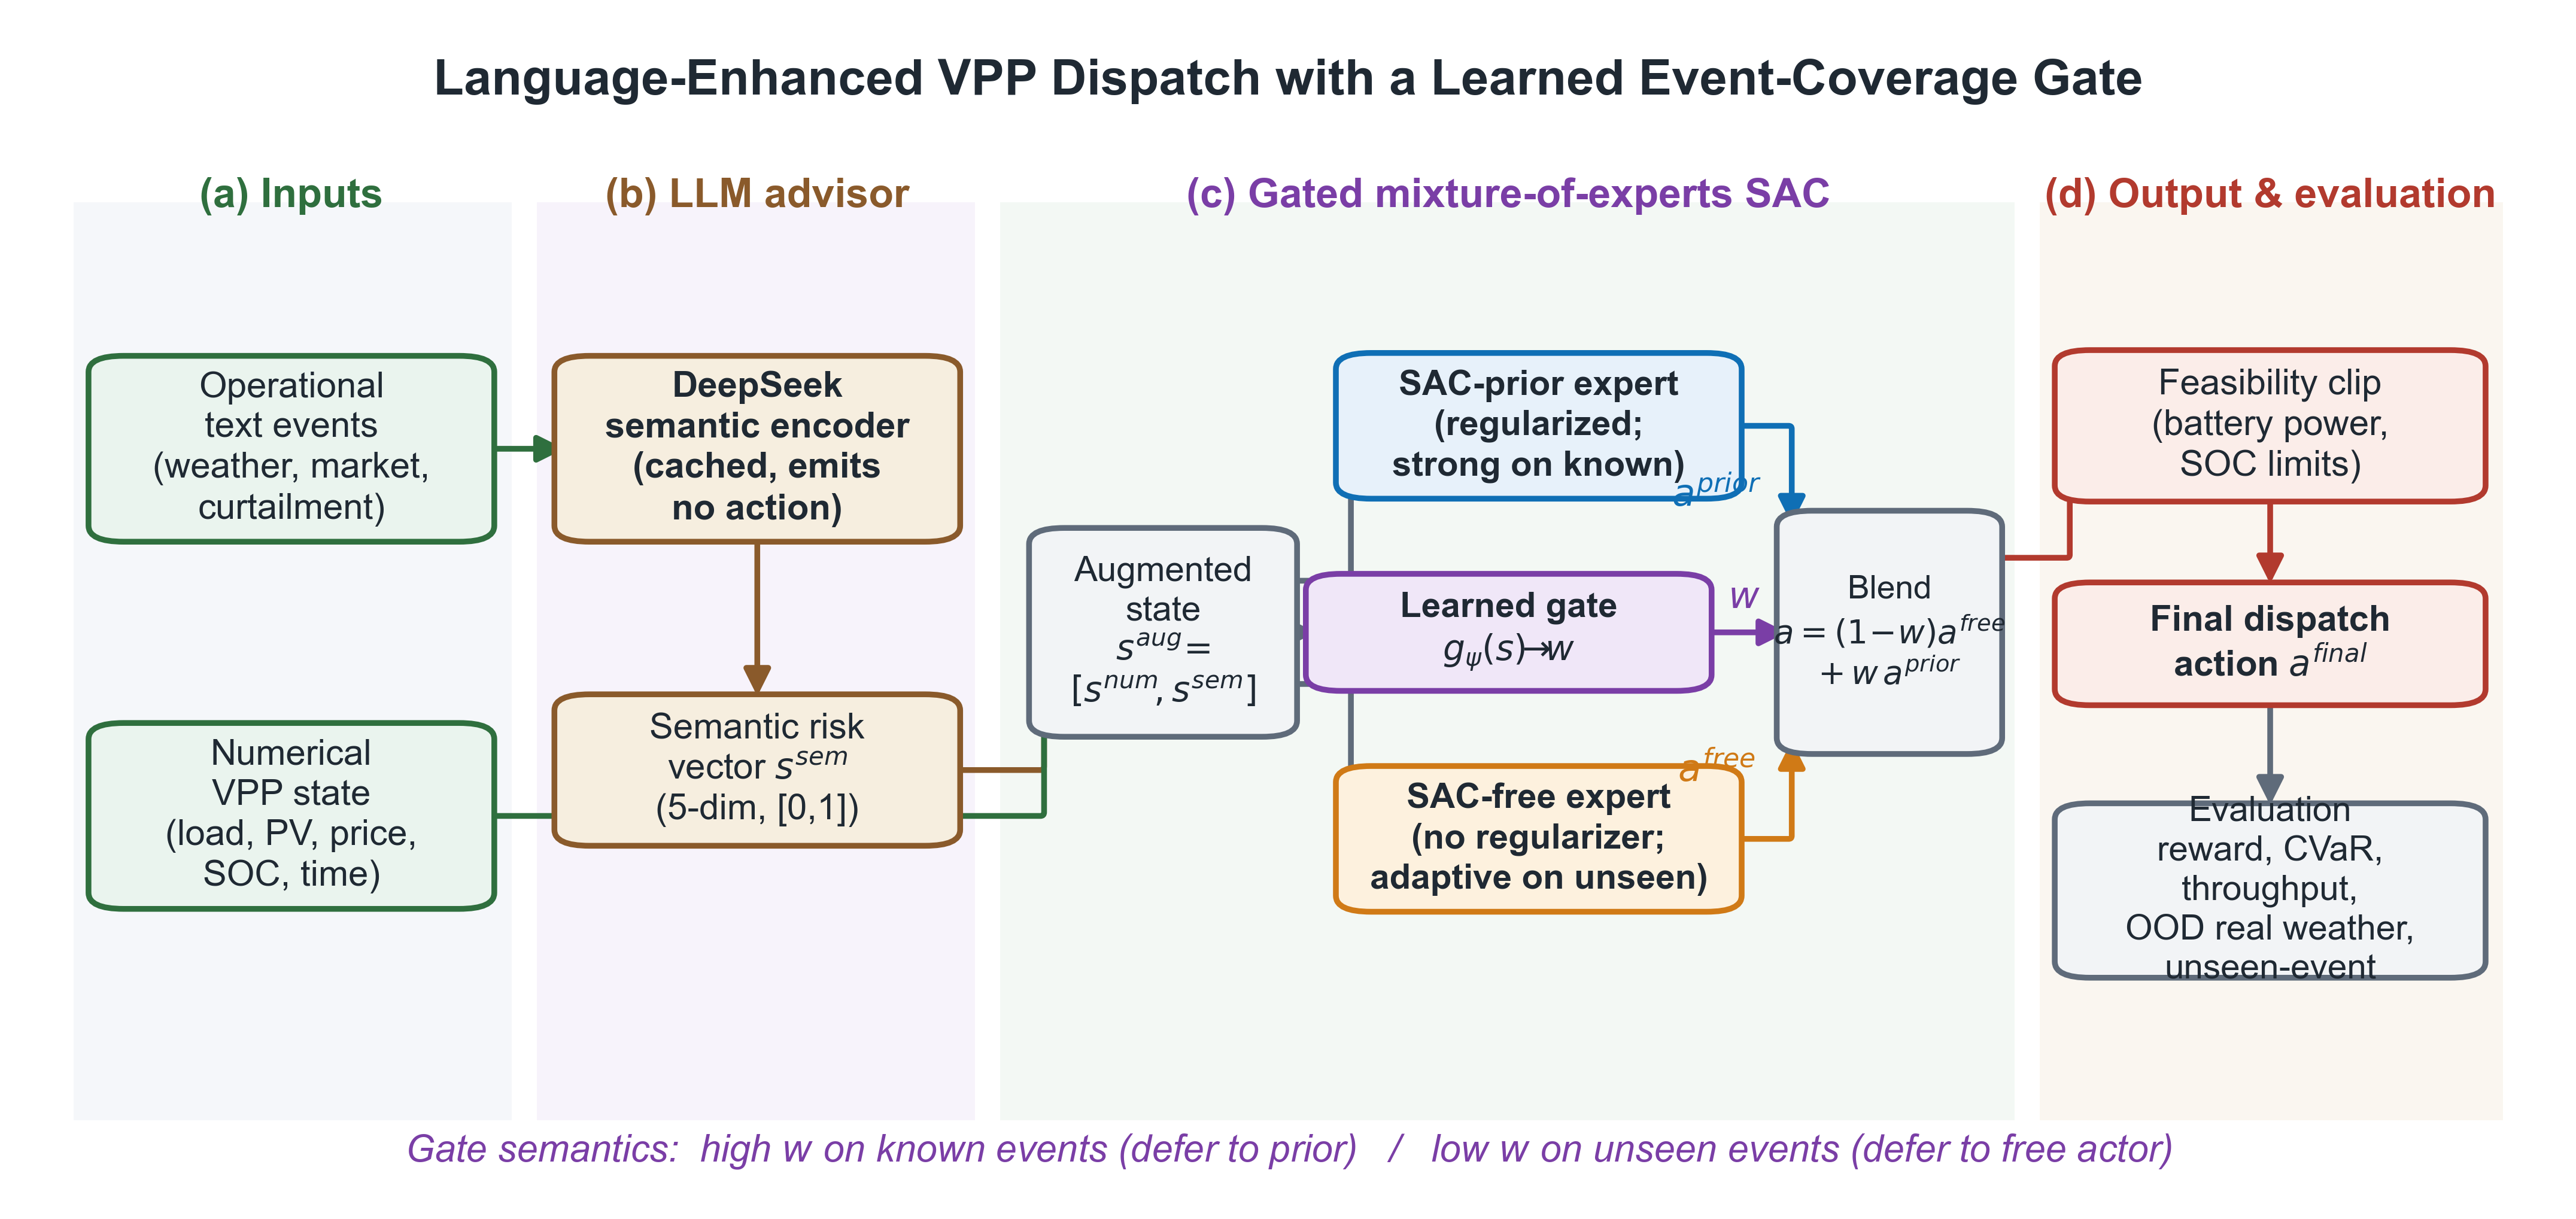
\includegraphics[width=0.92\linewidth]{figures/ieee_vpp_ledrl_architecture.png}
  \caption{Language-enhanced VPP dispatch framework with a learned event-coverage gate. (a) Event text and numerical VPP state inputs. (b) DeepSeek maps operational text to a cached semantic risk vector and never emits a dispatch action; the LLM serves as an advisor. (c) The augmented state drives two SAC experts---a regularized prior expert (strong on known events) and a free expert (adaptive on new or held-out negative-price events)---and a learned gate $g_\psi(s)\to w\in[0,1]$ blends their actions as $a=(1-w)a^{\mathrm{free}}+w a^{\mathrm{prior}}$. The gate is trained on per-batch-normalized $Q$-differences and recovers a high $w$ on known events and a low $w$ on negative-price events without coverage labels (Section~\ref{sec:gated_moe}); the two fixed configurations $w=0.9$ (known events) and $w=0$ with a relaxed regularizer (new-event adaptation) are the hand-set instances of the same principle (Sections~\ref{sec:method}--\ref{sec:unseen_event}). (d) The final action is clipped by battery feasibility and evaluated by reward, CVaR, throughput, an out-of-distribution real-weather test, and new-event adaptation tests.}
  \label{fig:architecture}
\end{figure*}

\subsection{LLM Semantic Encoder}
\label{sec:llm_encoder}
The semantic encoder is implemented with a DeepSeek large language model accessed through an OpenAI-compatible chat-completions interface. For each distinct operational event template (for example, a high-temperature warning or a renewable-curtailment notice), the encoder receives the event text together with the current temperature and price as context, and is prompted to return a JSON object containing the five risk scores $(r_t^{\mathrm{risk}}, r_t^{\mathrm{price}}, r_t^{\mathrm{load}}, r_t^{\mathrm{cur}}, b_t^{\mathrm{storage}})$ together with a short natural-language explanation. The returned scores are clamped to $[0,1]$ for the four risk dimensions and to $[-1,1]$ for the storage-bias signal. Because the encoder is queried only once per distinct event template and the results are cached, the language model does not participate in the per-step control loop and introduces no online inference latency; the SAC actor and safety layer consume the cached scores as static state features. The implementation also supports a local keyword-based encoder as a fallback when the API is unavailable. The reported experiments compare DeepSeek-derived semantic features with zeroed semantic features and numeric-safety-layer ablations; a dedicated DeepSeek-versus-keyword and noisy-score comparison remains necessary before making a strong claim that the gain is unique to LLM understanding rather than to structured text-derived features in general. The language model is never asked to emit a dispatch action, so the final decision remains deterministic, auditable, and physically constrained.

\subsection{SAC Decision Layer and Semantic Safety Layer}
SAC learns a stochastic actor $\pi_\theta(a_t|s_t)$ and two critic functions. The standard maximum-entropy actor objective is
\begin{equation}
J_{\pi} =
\mathbb{E}_{s_t \sim \mathcal{D}, a_t \sim \pi_\theta}
\left[
\alpha \log \pi_\theta(a_t|s_t)
- \min_{i=1,2} Q_{\phi_i}(s_t,a_t)
\right],
\end{equation}
where $\alpha$ is the entropy temperature and $\mathcal{D}$ is the replay buffer.

For LE-DRL-SAC, the state is $s^{\mathrm{aug}}_t$. To ensure that the semantic features influence learning, the actor objective is augmented with a semantic-consistency term:
\begin{equation}
J_{\pi}^{\mathrm{LE}} =
J_{\pi}
+ \lambda_{\mathrm{sem}}
\mathbb{E}\left[
\| a_t - a^{\mathrm{sem}}(s^{\mathrm{aug}}_t) \|^2
\right],
\end{equation}
where $a^{\mathrm{sem}}(\cdot)$ is a reference action direction derived from price, SOC, and risk features. High price-spike or load-pressure scores encourage discharging or preserving energy for peak periods, while renewable-curtailment pressure encourages charging during PV-surplus periods.

In the final policy, this same risk-consistent action prior is used as a deterministic semantic safety layer:
\begin{equation}
a^{\mathrm{final}}_t =
(1-w)a^{\mathrm{SAC}}_t + w a^{\mathrm{sem}}_t,
\end{equation}
where $w \in [0,1]$ is the safety-layer blending weight. The final action is then clipped by the battery power and SOC feasibility limits. This layer does not allow the language model to output arbitrary dispatch commands; it only maps structured risk scores into a bounded charging/discharging correction. The weight $w$ is treated as an event-coverage-dependent quantity rather than a universal constant: on event categories used to design the prior, the prior is close to scenario-optimal and a high $w$ is preferred; on event categories absent from prior design, the prior has no matching branch and a low $w$ lets the learned actor take over. In the main experiment on the four known-event scenarios, $w=0.9$ is selected from a prior-weight sweep because it outperforms all implemented baselines, including the rule-based controller, while retaining a nonzero learned SAC component; the semantic prior amplitude is bounded by a guidance power of $2.0$ MW. Section~\ref{sec:unseen_event} examines the complementary regime---a new negative-price event category introduced during adaptation---and reports a configuration in which $w$ is set to zero and the semantic-consistency regularizer is relaxed so that the learned actor, advised by the LLM-derived features, produces the final action. The two configurations together instantiate the event-coverage principle; the transition between them is later automated by a learned gate in Section~\ref{sec:gated_moe}. To isolate the contribution of textual semantics from the safety-layer mechanism itself, we also evaluate a diagnostic variant that replaces the semantic prior with a purely numeric prior $a^{\mathrm{num}}_t$ derived from price, SOC, hour, and PV surplus only; the same blending formula yields a numeric safety layer used only as an ablation baseline, not as the final controller.

The overall training and inference procedure is summarized in Algorithm~\ref{alg:ledrl}. Training proceeds in two offline stages---LLM caching and SAC learning---and inference applies the semantic safety layer on top of the learned actor, so the LLM is never invoked at deployment time.

\begin{algorithm}[t!]
\caption{LE-DRL-SAC Training and Semantic-Safety-Layer Inference}
\label{alg:ledrl}
\begin{algorithmic}[1]
\Require event templates $\mathcal{E}$, LLM encoder $\mathrm{LLM}(\cdot)$, empty cache $\mathcal{C}$
\Require semantic regularizer weight $\lambda_{\mathrm{sem}}$, safety weight $w$, guidance power $P_{\mathrm{guide}}$
\State \textbf{// Stage 1: offline LLM caching (one query per distinct event template)}
\For{each distinct template $e \in \mathcal{E}$}
    \State $(r^{\mathrm{risk}}, r^{\mathrm{price}}, r^{\mathrm{load}}, r^{\mathrm{cur}}, b^{\mathrm{storage}}) \gets \mathrm{LLM}(e)$
    \State clamp risk scores to $[0,1]$, storage bias to $[-1,1]$
    \State $\mathcal{C}[e] \gets s^{\mathrm{sem}}$ \Comment{cached; no LLM call at runtime}
\EndFor
\State \textbf{// Stage 2: SAC training with semantic-consistency regularization}
\State initialize actor $\pi_\theta$, critics $Q_{\phi_1}, Q_{\phi_2}$, replay buffer $\mathcal{D}$
\For{each training episode}
    \For{each 15-min step $t$}
        \State observe $s^{\mathrm{num}}_t$ and event template $e_t$; load $s^{\mathrm{sem}}_t \gets \mathcal{C}[e_t]$
        \State $s^{\mathrm{aug}}_t \gets [s^{\mathrm{num}}_t, s^{\mathrm{sem}}_t]$
        \State sample $a_t \sim \pi_\theta(\cdot \mid s^{\mathrm{aug}}_t)$
        \State clip $a_t$ by battery power/SOC feasibility; execute; observe $r_t, s^{\mathrm{num}}_{t+1}$
        \State store $(s^{\mathrm{aug}}_t, a_t, r_t, s^{\mathrm{aug}}_{t+1})$ in $\mathcal{D}$
        \State sample minibatch from $\mathcal{D}$; update critics by TD targets
        \State update $\pi_\theta$ by $\nabla_\theta \big[ \alpha \log \pi_\theta - \min_i Q_{\phi_i} + \lambda_{\mathrm{sem}}\|a_t - a^{\mathrm{sem}}(s^{\mathrm{aug}}_t)\|^2 \big]$
    \EndFor
\EndFor
\State \textbf{// Stage 3: inference with the semantic safety layer}
\Function{Dispatch}{$s^{\mathrm{num}}_t, e_t$}
    \State $s^{\mathrm{sem}}_t \gets \mathcal{C}[e_t]$;\ \ $s^{\mathrm{aug}}_t \gets [s^{\mathrm{num}}_t, s^{\mathrm{sem}}_t]$
    \State $a^{\mathrm{SAC}}_t \gets \pi_\theta(s^{\mathrm{aug}}_t)$ \Comment{deterministic mean}
    \State $a^{\mathrm{sem}}_t \gets$ risk-consistent prior, amplitude $\leq P_{\mathrm{guide}}$
    \State $a^{\mathrm{final}}_t \gets (1-w)\,a^{\mathrm{SAC}}_t + w\,a^{\mathrm{sem}}_t$
    \State \Return clip($a^{\mathrm{final}}_t$) by battery feasibility
\EndFunction
\end{algorithmic}
\end{algorithm}

\subsection{Compared Policies}
The following policies are evaluated:
\begin{itemize}
  \item \textbf{SAC-Numeric}: SAC using numerical state only.
  \item \textbf{LE-DRL w/o Text}: same input dimension as LE-DRL-SAC, but semantic features are set to zero.
  \item \textbf{LE-DRL-SAC}: language-enhanced SAC without test-time safety blending.
  \item \textbf{LE-DRL-SAC + semantic safety layer}: final proposed controller with $w=0.9$.
  \item \textbf{Rule-Based}: deterministic threshold policy using price, PV surplus, time, and SOC.
  \item \textbf{Rolling-Horizon}: solver-free rolling-horizon dynamic-programming optimizer with a 16-step horizon, discrete action grid, and SOC grid. It is a strong operational benchmark with short-horizon look-ahead.
  \item \textbf{Enhanced Rolling-Horizon}: an engineering-regularized MPC-like rolling optimizer that augments the rolling-horizon baseline with a terminal SOC value, an action-smoothing penalty, and an additional cycling penalty. It is reported alongside the original rolling-horizon optimizer to expose the throughput--reward trade-off of aggressive short-horizon optimization.
  \item \textbf{Linear-MPC}: a receding-horizon linear-programming baseline (Scipy HiGHS, 24-step horizon, terminal SOC penalty) that solves a deterministic LP at each step under explicit SOC, power, and curtailment constraints.
  \item \textbf{SAC-Numeric + numeric safety layer}: a diagnostic variant of SAC-Numeric in which the learned action is blended with a purely numeric safety prior $a^{\mathrm{num}}_t$ using the same blending formula as the semantic safety layer but without any textual information. It isolates the value of the safety-layer mechanism from the value of language-derived semantics.
  \item \textbf{Random and Soft-Q}: weak and transitional baselines used for diagnostic comparison.
\end{itemize}

\section{Experimental Setup}
\label{sec:experiment}

Four seven-day scenarios are evaluated:
\begin{itemize}
  \item S1: normal summer operation.
  \item S2: high-temperature load pressure.
  \item S3: price-spike event.
  \item S4: renewable-curtailment pressure.
\end{itemize}

SAC-Numeric, LE-DRL w/o Text, and LE-DRL-SAC are trained for 80 episodes with seeds 2026, 2031, and 2042 for the main cross-scenario comparison on S1--S4. LE-DRL-SAC uses LLM-derived semantic features in the current experiment, with semantic auxiliary reward scale 0.35 and actor semantic-consistency weight 3.0. After training, the semantic safety-layer weight is swept over $w \in \{0,0.25,0.50,0.75,0.85,0.90,1.00\}$ to quantify the trade-off between learned actor control and deterministic semantic correction. The main controller uses $w=0.9$ with a semantic guidance power of $2.0$ MW; $w=0$ corresponds to the learned LE-DRL-SAC actor without test-time semantic safety blending, and $w=1$ corresponds to the semantic safety prior alone. The new-event adaptation study and the parameter-variant study (Sections~\ref{sec:unseen_event}--\ref{sec:gated_moe}) extend the training set to S1--S5 and use five seeds (2026, 2031, 2042, 2047, 2053) to strengthen the statistical evidence on the negative-price event category and its held-out variants.

The main metrics comprise total reward, average step reward, CVaR 5\%, final SOC, battery throughput, high-price discharge rate, and low-price charge rate. Higher total reward and less-negative CVaR are preferred. The high-price discharge rate and low-price charge rate serve as behavioral indicators rather than direct optimization objectives.

\section{Results and Discussion}
\label{sec:results}

\subsection{Cross-Scenario Baseline Comparison}
Table~\ref{tab:baseline_summary} summarizes the cross-scenario results. The final LE-DRL-SAC controller with the semantic safety layer ($w=0.9$) achieves the best average total reward among the implemented methods. It improves the average total reward from -211,023.2 yuan for SAC-Numeric to -208,468.9 yuan and also exceeds the deterministic Rule-Based controller (-208,969.9 yuan), the engineering-regularized Enhanced Rolling-Horizon optimizer (-209,988.3 yuan), the Linear-MPC baseline (-210,656.0 yuan), and the diagnostic SAC-Numeric with a numeric safety layer (-209,125.3 yuan). The result is not obtained by weakening the baselines: the comparison includes a rule-based controller, an aggressive rolling-horizon optimizer, an engineering-regularized enhanced rolling-horizon optimizer, a Linear-MPC receding-horizon optimizer, a text-ablation SAC, a numeric-safety-layer SAC, and the pure LE-DRL-SAC actor without test-time safety blending.

The comparison also clarifies the role of the safety layer. Pure LE-DRL-SAC improves substantially over SAC-Numeric, but its average reward (-210,447.8 yuan in the 80-episode run) remains below the strongest rule baseline. Adding the safety layer gives the learned actor a bounded event-aware correction and closes this operational gap. Notably, the numeric safety layer already improves SAC-Numeric from -211,023.2 to -209,125.3 yuan, which confirms that the safety-layer mechanism itself carries value; however, the semantic safety layer still achieves -208,468.9 yuan, beyond the numeric-safety-layer variant, indicating that structured text-derived semantic features contribute additional value on top of the mechanism. This comparison should not be interpreted as evidence that the learned actor alone is the strongest known-event controller; on S1--S4, the hand-crafted prior carries much of the in-sample benefit, and the actor's distinct role is exposed more clearly in the new-event adaptation and gate analyses. The Enhanced Rolling-Horizon optimizer reduces average battery throughput from 133.16 MWh of the original rolling-horizon baseline to 14.80 MWh at the cost of slightly lower reward, reflecting a more conservative but engineering-plausible operational policy.

\begin{table*}[t!]
\caption{Cross-Scenario Summary of Main Baselines}
\label{tab:baseline_summary}
\centering
\begin{tabular}{lccccc}
\toprule
\textbf{Model} & \textbf{Total reward (yuan)} $\uparrow$ & \textbf{CVaR 5\% (yuan)} $\uparrow$ & \textbf{Throughput (MWh)} & \textbf{High-price discharge} & \textbf{Low-price charge} \\
\midrule
LE-DRL-SAC + safety layer ($w=0.9$) & \textbf{-208,468.9} & \textbf{-696.7} & 28.37 & 0.231 & 0.185 \\
Rule-Based & -208,969.9 & -705.0 & 19.94 & 0.176 & 0.113 \\
SAC-Numeric + numeric safety layer & -209,125.3 & -704.0 & 16.92 & 0.193 & 0.167 \\
LE-DRL-SAC, actor only ($w=0$) & -210,447.8 & -697.1 & 14.35 & \textbf{0.501} & 0.129 \\
Enhanced Rolling-Horizon & -209,988.3 & -713.8 & 14.80 & 0.095 & 0.042 \\
Linear-MPC & -210,656.0 & -714.6 & 10.81 & 0.073 & 0.101 \\
Rolling-Horizon & -210,616.7 & -731.6 & 133.16 & 0.436 & \textbf{0.943} \\
SAC-Numeric & -211,023.2 & -721.3 & 3.04 & 0.000 & 0.000 \\
LE-DRL w/o Text & -211,023.1 & -721.3 & 3.04 & 0.000 & 0.000 \\
\bottomrule
\end{tabular}
\end{table*}

\subsection{Scenario-Level Results}
Table~\ref{tab:scenario_results} reports the core scenario-level comparison. The proposed controller obtains the best total reward in S1, S2, and S4. In S3, Linear-MPC attains the highest total reward, while the proposed controller remains the best non-optimization-learning controller and exceeds Rolling-Horizon with far lower battery throughput. The SAC-Numeric + numeric safety layer variant and the Linear-MPC baseline are strong optimization references, confirming that a receding-horizon optimizer with explicit constraints provides competitive event-responsive behavior; however, the language-enhanced controller still exceeds both on the cross-scenario average. The Enhanced Rolling-Horizon optimizer achieves low battery throughput in every scenario, illustrating the engineering-regularized trade-off between cycling cost and economic reward.

\begin{figure}[t!]
  \centering
  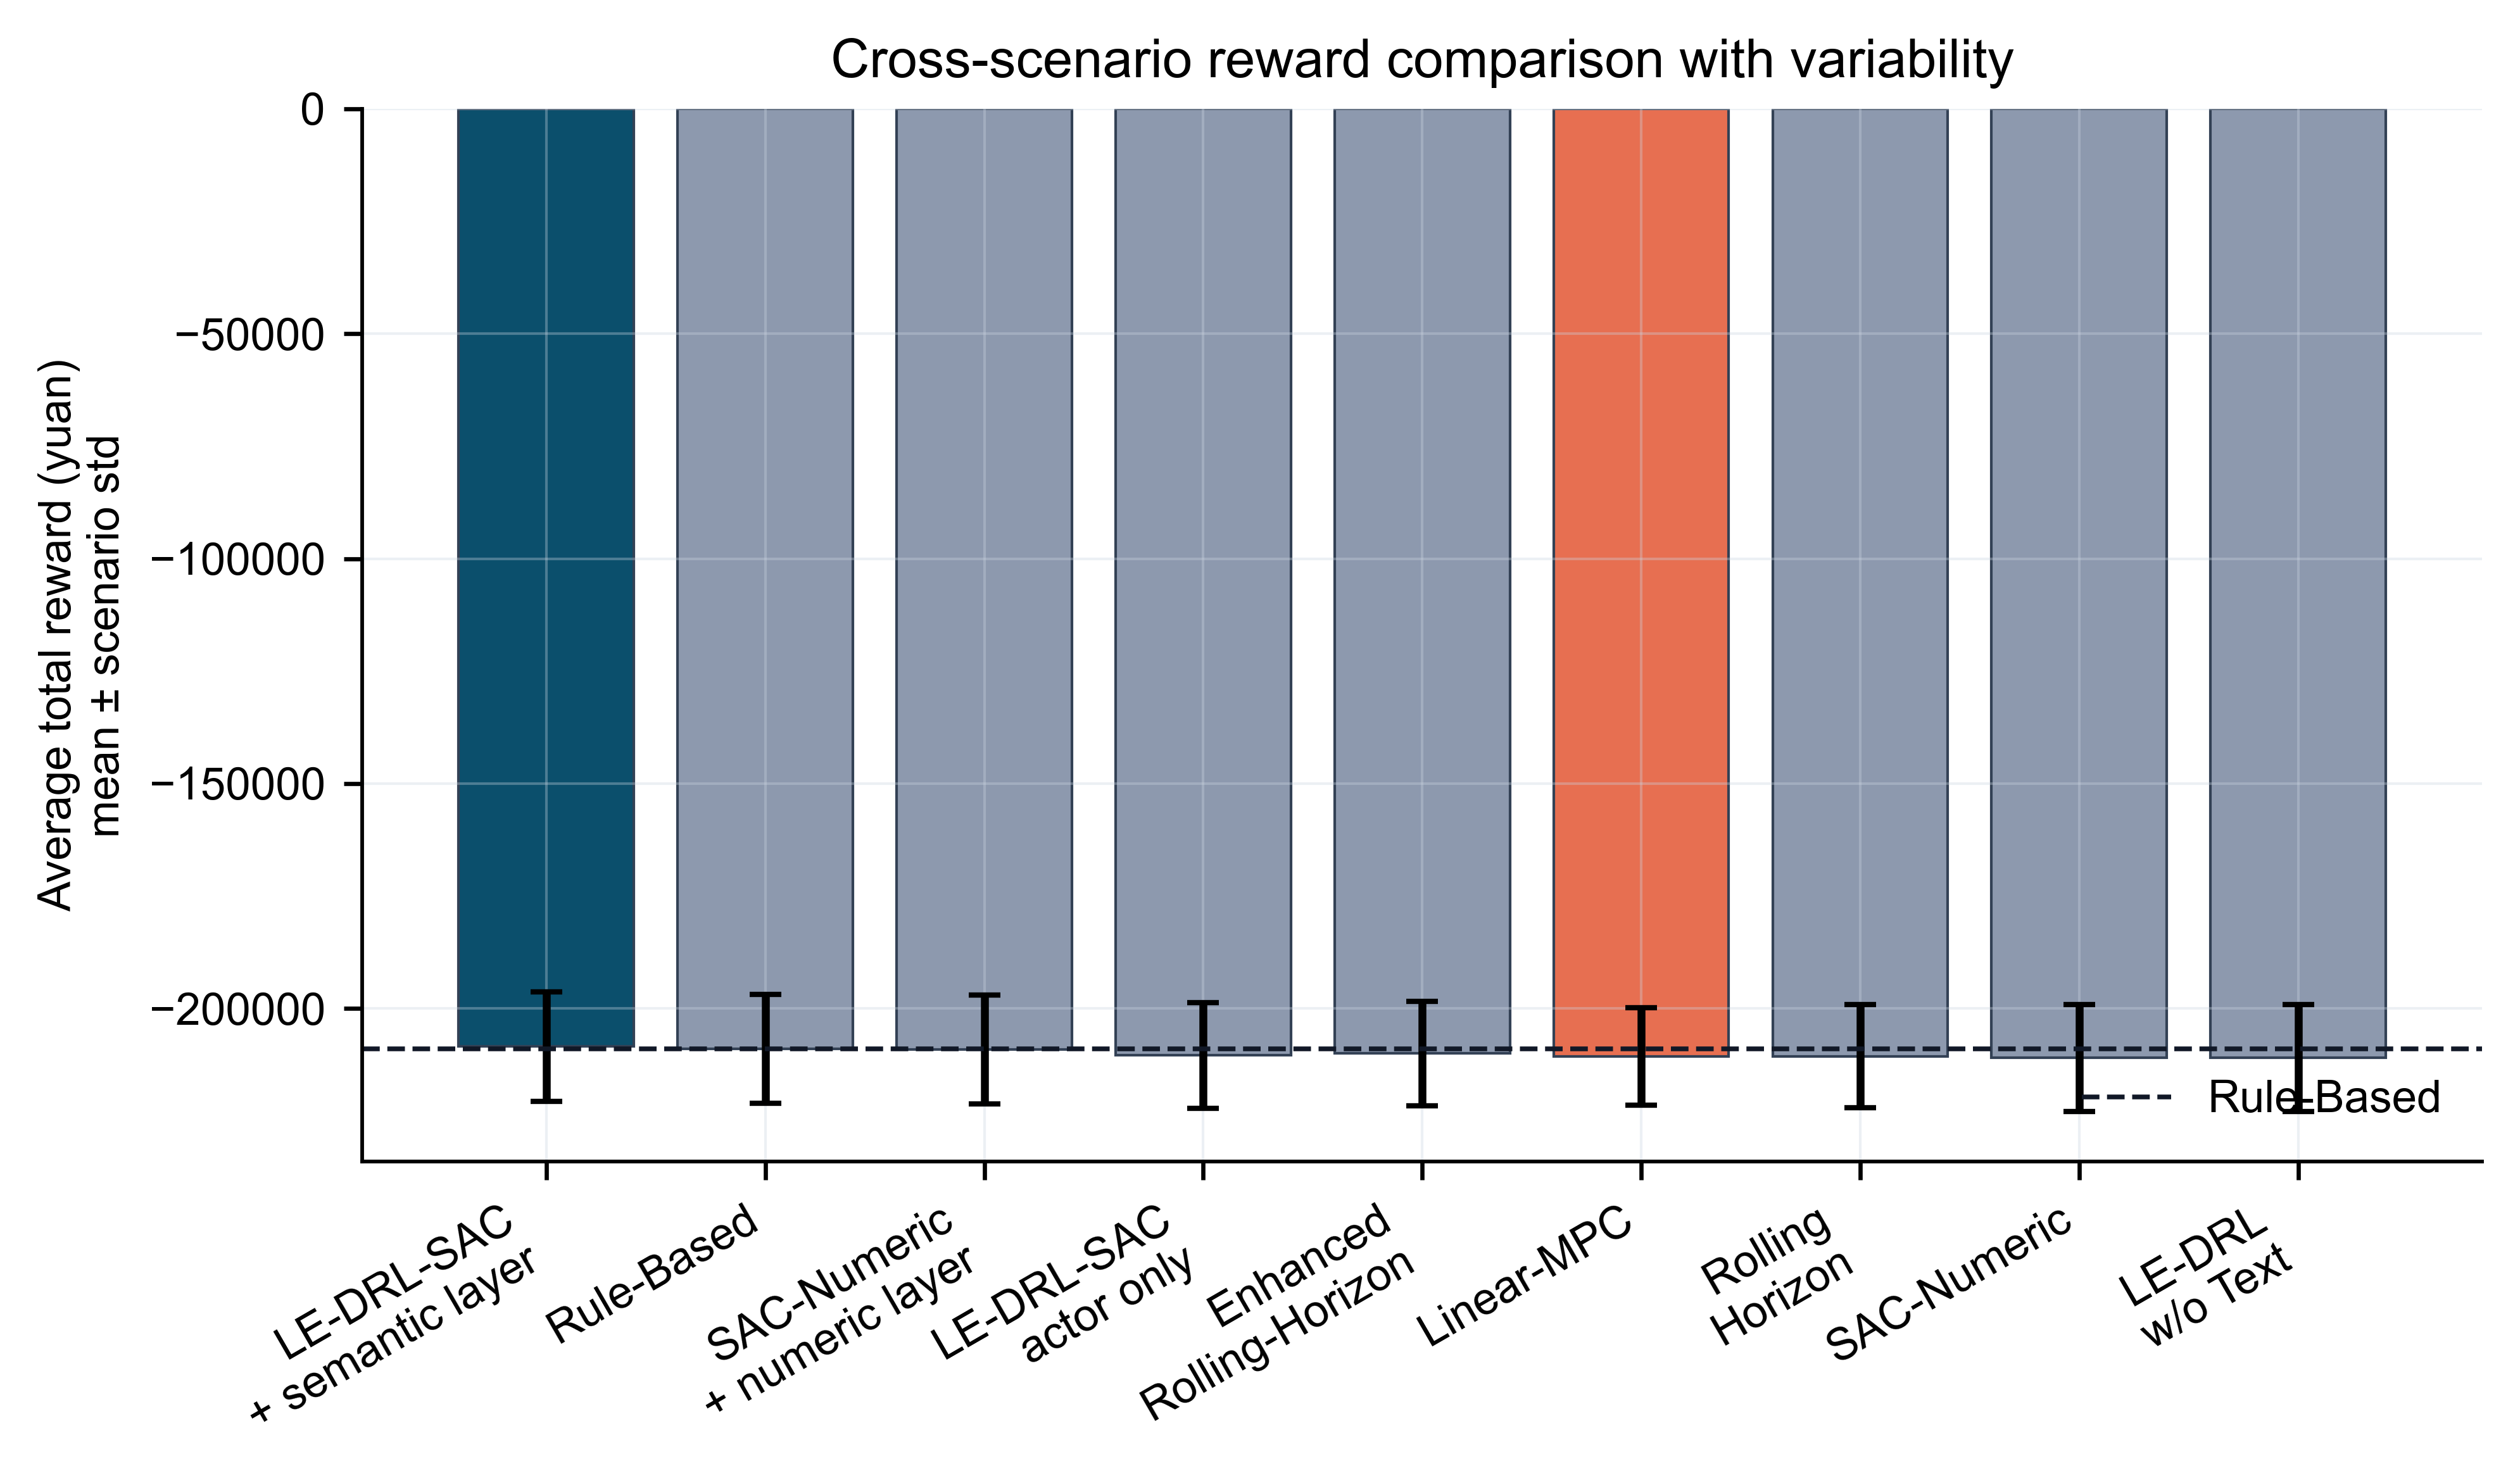
\includegraphics[width=0.98\columnwidth]{figures/baseline_reward_with_error.png}
  \caption{Cross-scenario average total reward with scenario variability (mean $\pm$ std). The dashed line marks the rule-based controller. The proposed LE-DRL-SAC with the semantic safety layer attains the highest average reward.}
  \label{fig:baseline_reward_error}
\end{figure}

\begin{figure}[t!]
  \centering
  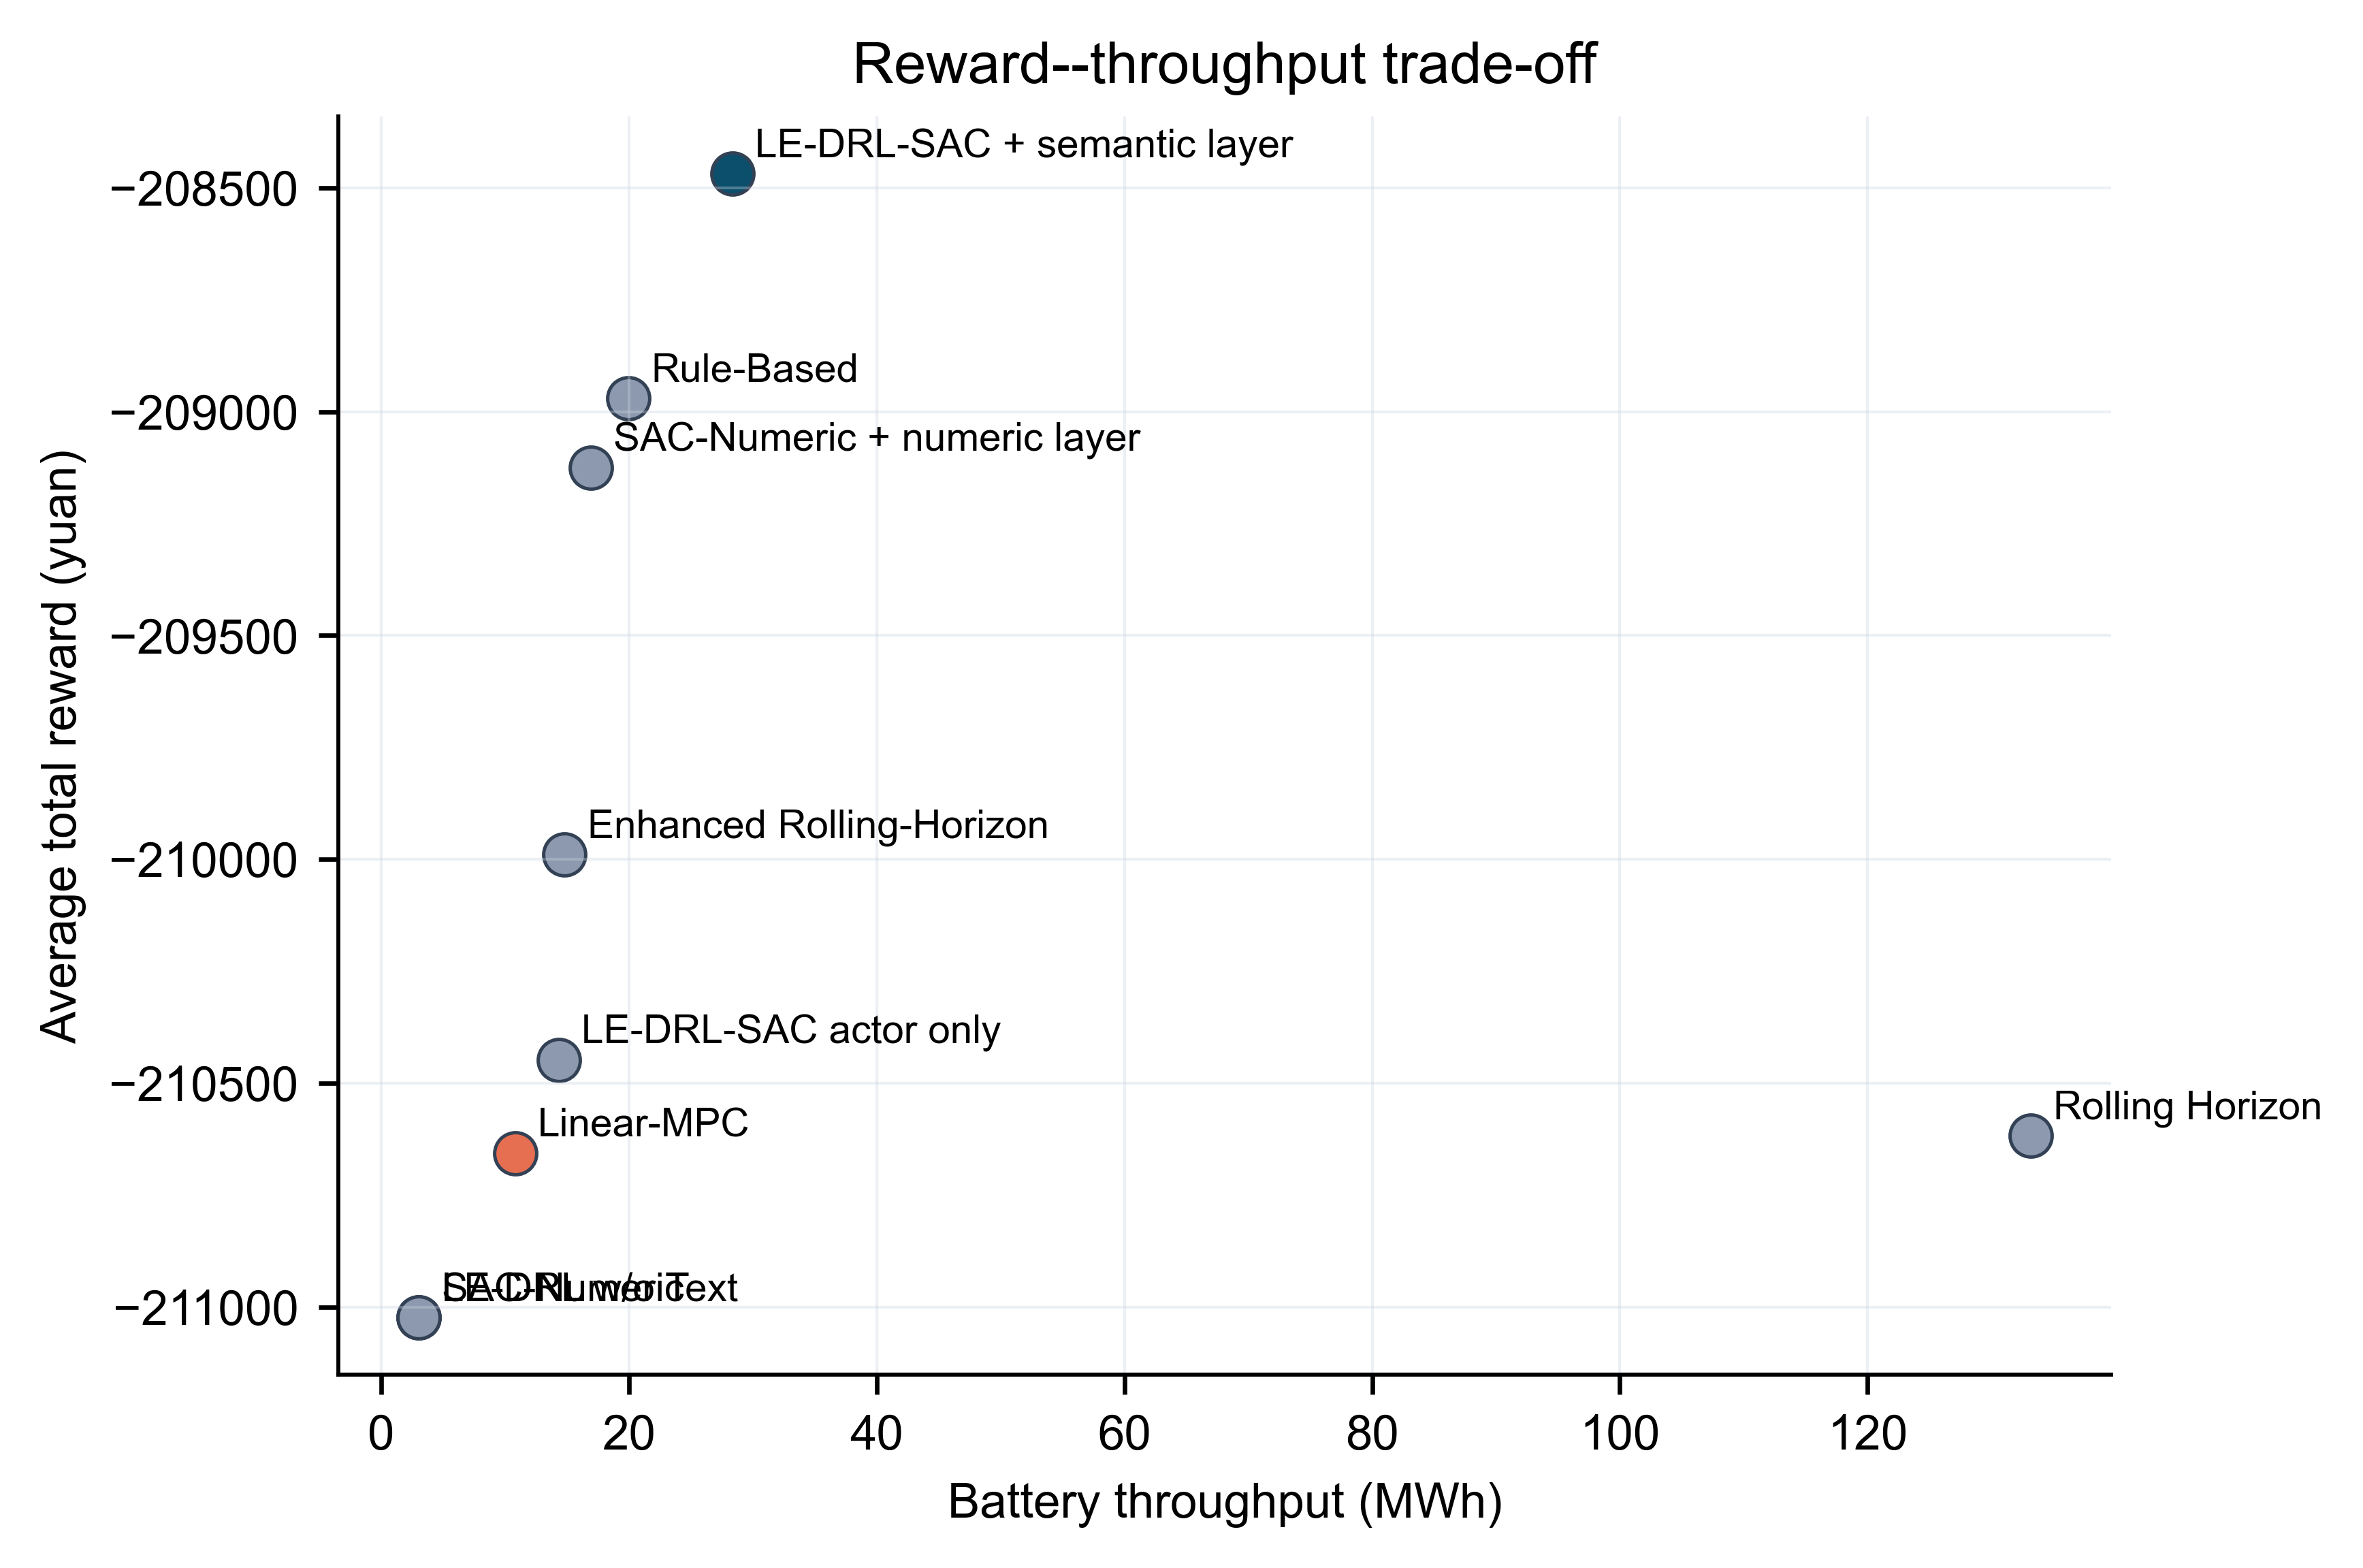
\includegraphics[width=0.98\columnwidth]{figures/reward_throughput_tradeoff.png}
  \caption{Reward--throughput trade-off across controllers. The aggressive rolling-horizon optimizer reaches competitive reward at the cost of excessive battery cycling (133 MWh), whereas the engineering-regularized Enhanced Rolling-Horizon and the proposed controller remain in a low-throughput, high-reward region.}
  \label{fig:tradeoff}
\end{figure}

\begin{table*}[t!]
\caption{Scenario-Level Comparison of Core Baselines}
\label{tab:scenario_results}
\centering
\begin{tabular}{llrrrr}
\toprule
\textbf{Scenario} & \textbf{Model} & \textbf{Total reward} & \textbf{CVaR 5\%} & \textbf{Throughput} & \textbf{High-price discharge} \\
\midrule
\multirow{9}{*}{S1} & LE-DRL-SAC + safety layer & \textbf{-201,654.0} & -644.5 & 25.30 & 0.222 \\
& SAC-Numeric + numeric safety layer & -202,002.9 & -650.5 & 15.68 & 0.202 \\
& Rule-Based & -202,010.4 & -652.1 & 16.96 & 0.161 \\
& LE-DRL-SAC, actor only & -203,160.8 & \textbf{-640.6} & 13.16 & \textbf{0.522} \\
& Enhanced Rolling-Horizon & -202,785.9 & -654.5 & 8.80 & 0.054 \\
& SAC-Numeric & -203,502.9 & -664.2 & 3.04 & 0.000 \\
& LE-DRL w/o Text & -203,502.8 & -664.2 & 3.04 & 0.000 \\
& Linear-MPC & -204,279.4 & -659.1 & 2.26 & 0.018 \\
& Rolling-Horizon & -204,122.5 & -655.8 & 133.65 & 0.429 \\
\midrule
\multirow{9}{*}{S2} & LE-DRL-SAC + safety layer & \textbf{-218,759.4} & -722.1 & 23.17 & 0.196 \\
& SAC-Numeric + numeric safety layer & -219,123.6 & -729.9 & 11.48 & 0.149 \\
& Rule-Based & -219,181.9 & -735.9 & 11.84 & 0.119 \\
& LE-DRL-SAC, actor only & -220,026.9 & \textbf{-719.4} & 12.56 & \textbf{0.462} \\
& Enhanced Rolling-Horizon & -219,984.3 & -734.7 & 5.60 & 0.030 \\
& SAC-Numeric & -220,257.2 & -740.1 & 3.04 & 0.000 \\
& LE-DRL w/o Text & -220,257.1 & -740.1 & 3.04 & 0.000 \\
& Linear-MPC & -221,276.2 & -736.9 & 0.45 & 0.018 \\
& Rolling-Horizon & -221,726.8 & -733.9 & 133.65 & 0.435 \\
\midrule
\multirow{9}{*}{S3} & LE-DRL-SAC + safety layer & -218,660.5 & -797.4 & 25.38 & 0.183 \\
& Rolling-Horizon & -218,749.2 & -880.2 & 131.17 & 0.458 \\
& Rule-Based & -219,146.3 & -802.0 & 18.80 & 0.155 \\
& LE-DRL-SAC, actor only & -220,815.3 & \textbf{-786.8} & 16.62 & \textbf{0.492} \\
& SAC-Numeric + numeric safety layer & -219,595.1 & -805.1 & 15.74 & 0.155 \\
& Enhanced Rolling-Horizon & -219,727.2 & -805.2 & 35.20 & 0.238 \\
& Linear-MPC & \textbf{-218,356.7} & -800.4 & 35.41 & 0.214 \\
& SAC-Numeric & -222,024.8 & -810.7 & 3.04 & 0.000 \\
& LE-DRL w/o Text & -222,024.7 & -810.7 & 3.04 & 0.000 \\
\midrule
\multirow{9}{*}{S4} & LE-DRL-SAC + safety layer & \textbf{-194,801.9} & \textbf{-622.6} & 39.61 & 0.323 \\
& Rule-Based & -195,541.0 & -630.0 & 32.16 & 0.268 \\
& SAC-Numeric + numeric safety layer & -195,779.9 & -630.3 & 24.76 & 0.268 \\
& Linear-MPC & -198,711.7 & -661.8 & 5.12 & 0.042 \\
& LE-DRL-SAC, actor only & -197,788.3 & -641.7 & 15.05 & \textbf{0.528} \\
& Enhanced Rolling-Horizon & -197,455.9 & -660.7 & 9.60 & 0.060 \\
& Rolling-Horizon & -197,868.2 & -656.6 & 134.16 & 0.423 \\
& SAC-Numeric & -198,308.3 & -670.2 & 3.04 & 0.000 \\
& LE-DRL w/o Text & -198,308.2 & -670.2 & 3.04 & 0.000 \\
\bottomrule
\end{tabular}
\end{table*}

\subsection{Semantic Safety-Layer Weight Sweep}
Table~\ref{tab:weight_sweep} reports the semantic safety-layer weight sweep. Increasing $w$ improves total reward on S1--S4 because the semantic prior provides direct event-responsive charging and discharging corrections for the event categories it was designed to cover. The main paper uses $w=0.9$, which outperforms all implemented baselines, including the rule-based controller, while retaining a nonzero learned SAC component. We acknowledge that $w=1.0$ yields a slightly higher reward (-208,278.4 yuan) than $w=0.9$ (-208,468.9 yuan); under $w=1.0$ the controller degenerates to the semantic prior alone and the SAC actor is no longer used at test time. This is an important boundary of the known-event result rather than a detail to hide: for S1--S4, the table primarily shows that the hand-crafted semantic prior is strong when event coverage is complete. We therefore report $w=1.0$ as an in-sample prior upper bound and retain $w=0.9$ as the main hybrid configuration for two reasons. First, the prior is a scenario-specific mapping designed with full knowledge of the four event categories; it cannot adapt without being rewritten. Second, in a real deployment, event categories and market conditions evolve, and the learned SAC component provides the adaptive capacity examined in the new-event adaptation and learned-gate studies. A pure prior cannot improve with additional data, whereas a hybrid controller can be fine-tuned or gated. The contribution should therefore be read as a coverage-dependent hybrid-control principle, not as a claim that the SAC actor alone dominates the known-event prior.

\begin{table}[t!]
\caption{Semantic Safety-Layer Weight Sweep}
\label{tab:weight_sweep}
\centering
\begin{tabular}{cccc}
\toprule
\textbf{$w$} & \textbf{Total reward} $\uparrow$ & \textbf{CVaR 5\%} $\uparrow$ & \textbf{Throughput} \\
\midrule
0.00 & -210,447.8 & \textbf{-697.1} & 14.35 \\
0.25 & -209,874.6 & -691.4 & 16.82 \\
0.50 & -209,330.5 & -692.5 & 21.23 \\
0.75 & -208,789.9 & -694.4 & 26.02 \\
0.85 & -208,599.0 & -695.9 & 27.51 \\
0.90 & -208,468.9 & -696.7 & 28.37 \\
1.00 & \textbf{-208,278.4} & -697.0 & 29.59 \\
\bottomrule
\end{tabular}
\end{table}

\begin{figure}[t!]
  \centering
  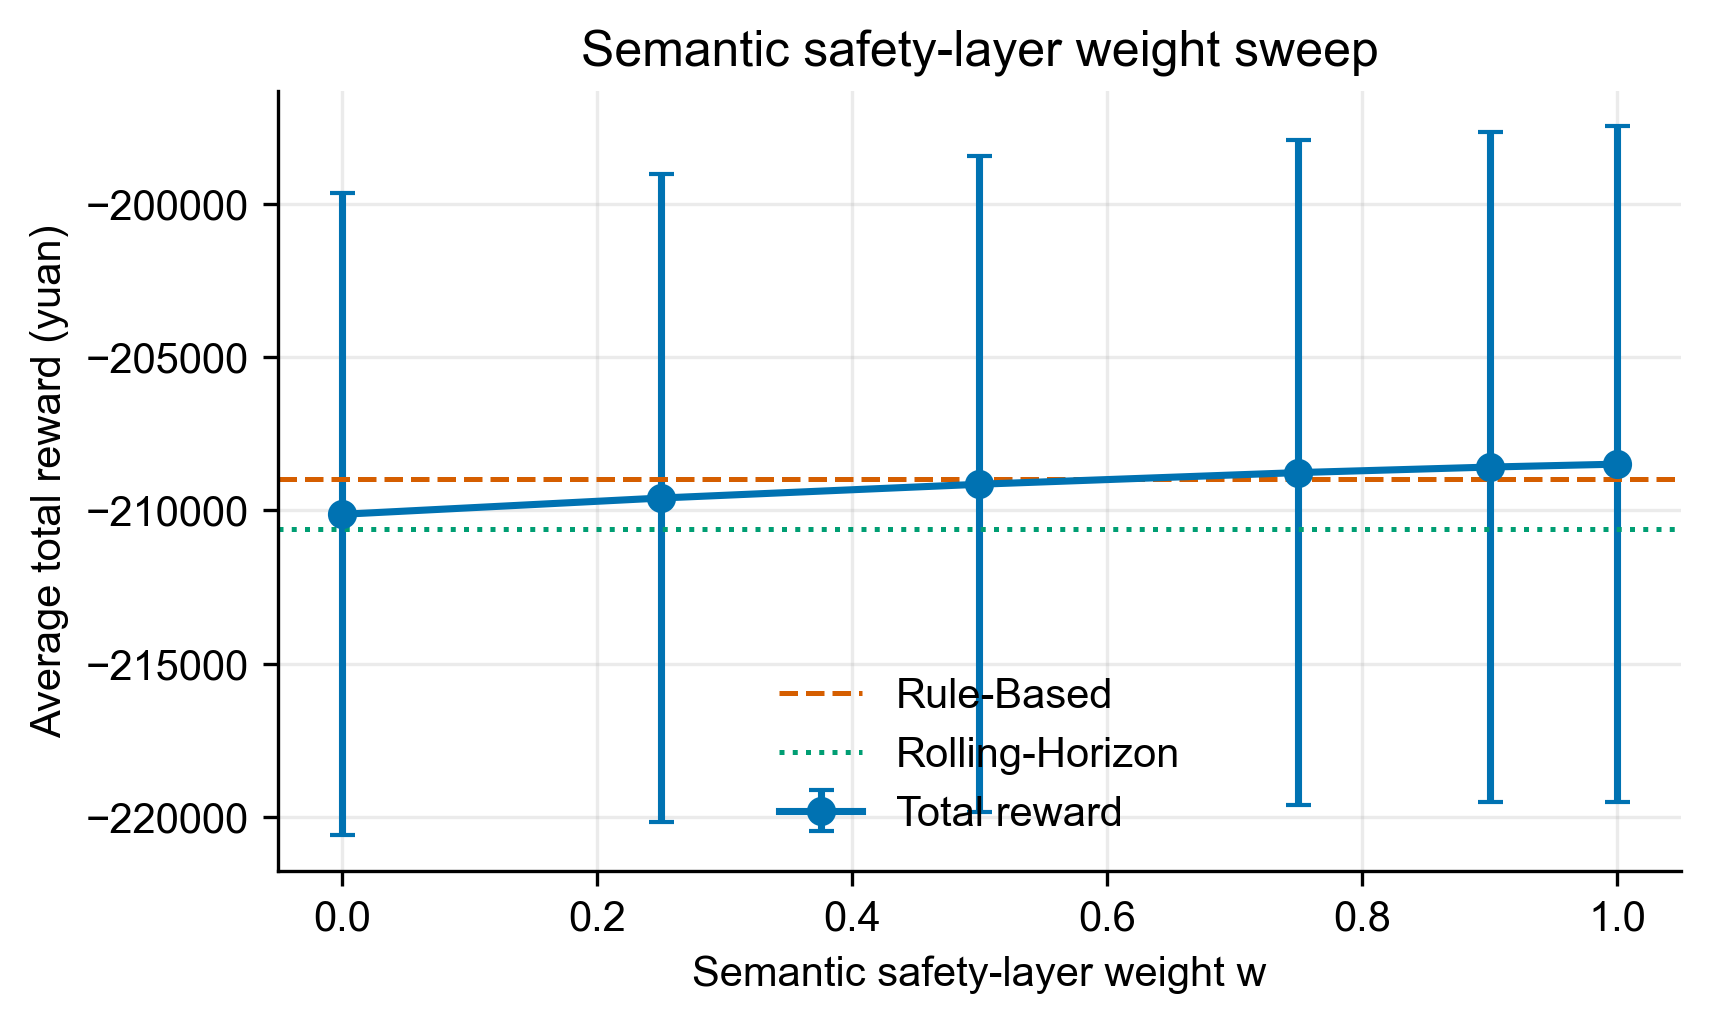
\includegraphics[width=0.98\columnwidth]{figures/semantic_safety_weight_sweep.png}
  \caption{Average total reward under different semantic safety-layer weights. The dashed and dotted reference lines indicate the Rule-Based and Rolling-Horizon baselines, respectively.}
  \label{fig:weight_sweep}
\end{figure}

\subsection{Training and Behavior Analysis}
Fig.~\ref{fig:training_curve} shows the training curves of SAC-Numeric, LE-DRL w/o Text, and LE-DRL-SAC. The language-enhanced actor forms a higher-reward evaluation trajectory in later episodes. Fig.~\ref{fig:total_reward} shows the scenario-level reward comparison of the trained SAC variants before adding the final safety-layer sweep. Fig.~\ref{fig:text_ablation} highlights the text-ablation result: SAC-Numeric and LE-DRL w/o Text are almost identical, while LE-DRL-SAC achieves higher reward after adding DeepSeek-derived semantic features.

\begin{figure}[t!]
  \centering
  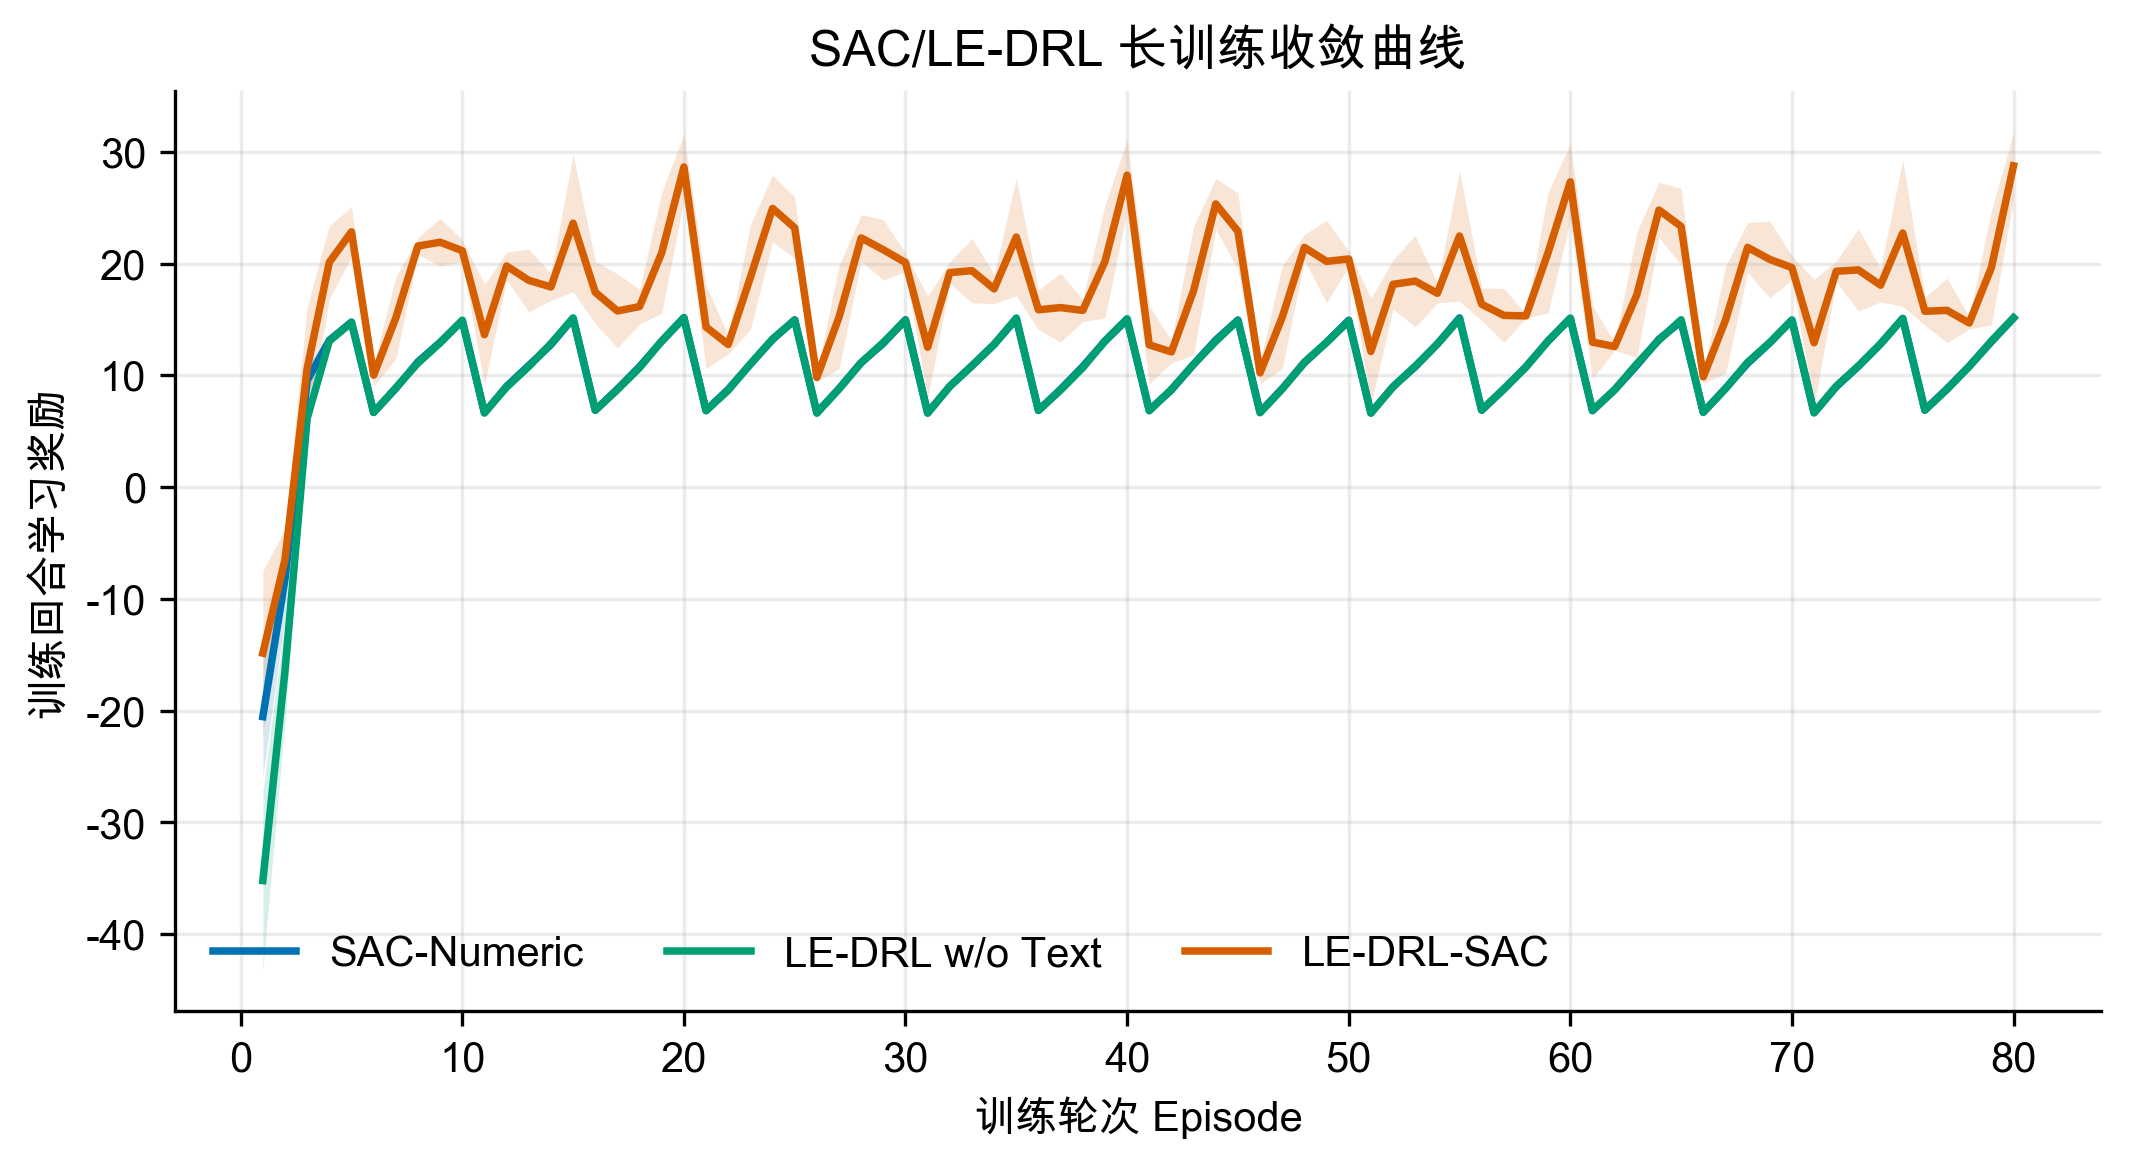
\includegraphics[width=0.98\columnwidth]{figures/training_curve.png}
  \caption{Training curves of SAC-Numeric, LE-DRL w/o Text, and LE-DRL-SAC under three random seeds.}
  \label{fig:training_curve}
\end{figure}

\begin{figure}[t!]
  \centering
  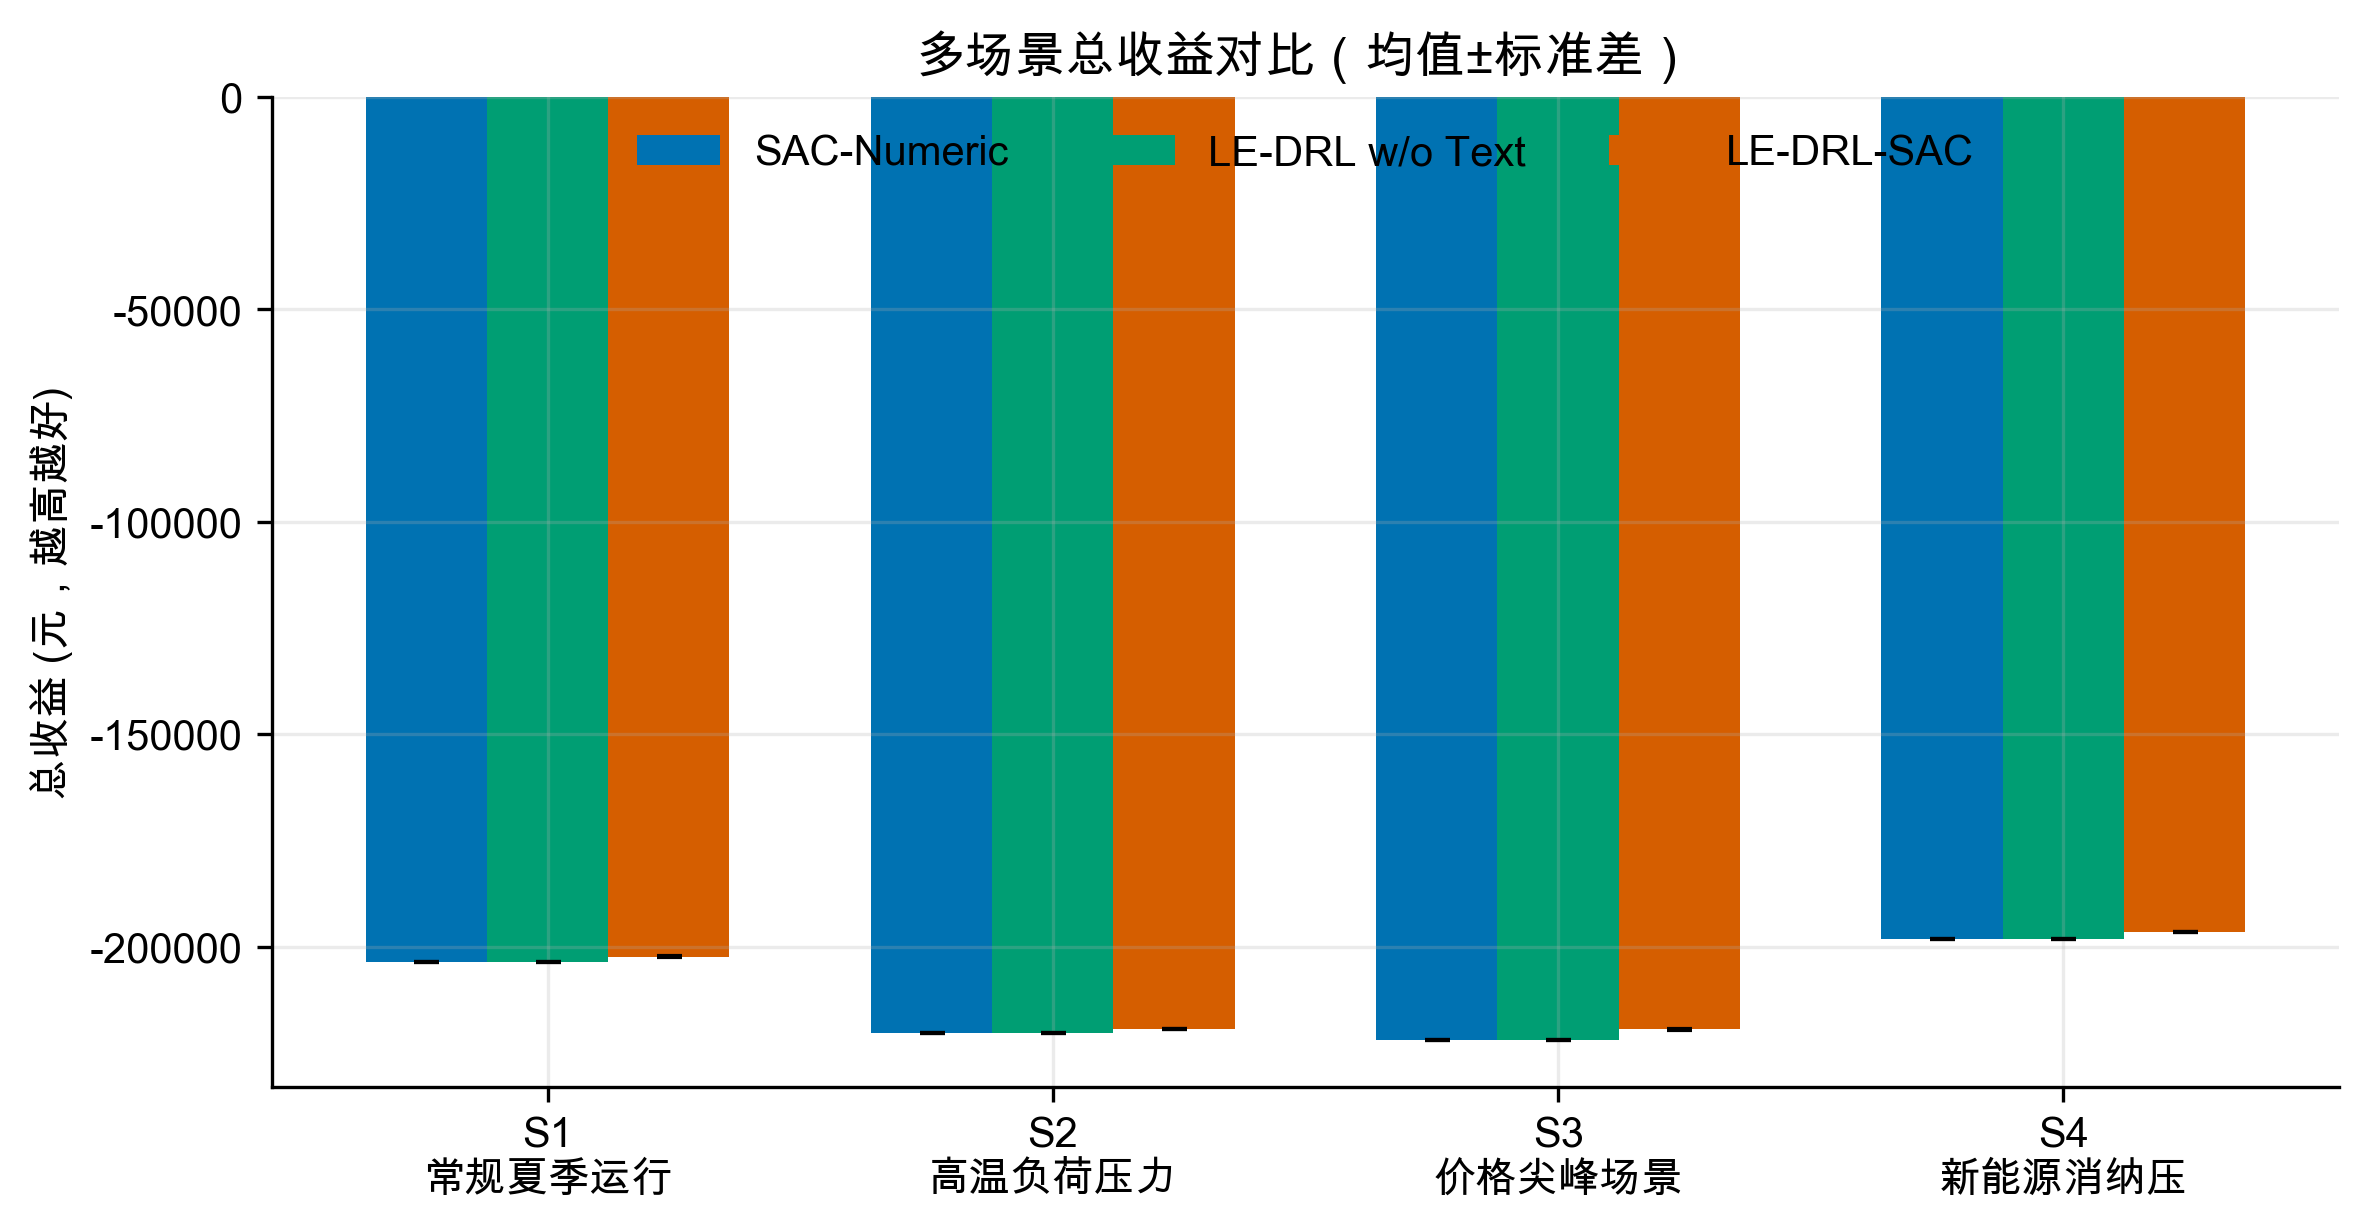
\includegraphics[width=0.98\columnwidth]{figures/scenario_total_reward.png}
  \caption{Scenario-level total reward comparison for the trained SAC variants.}
  \label{fig:total_reward}
\end{figure}

\begin{figure}[t!]
  \centering
  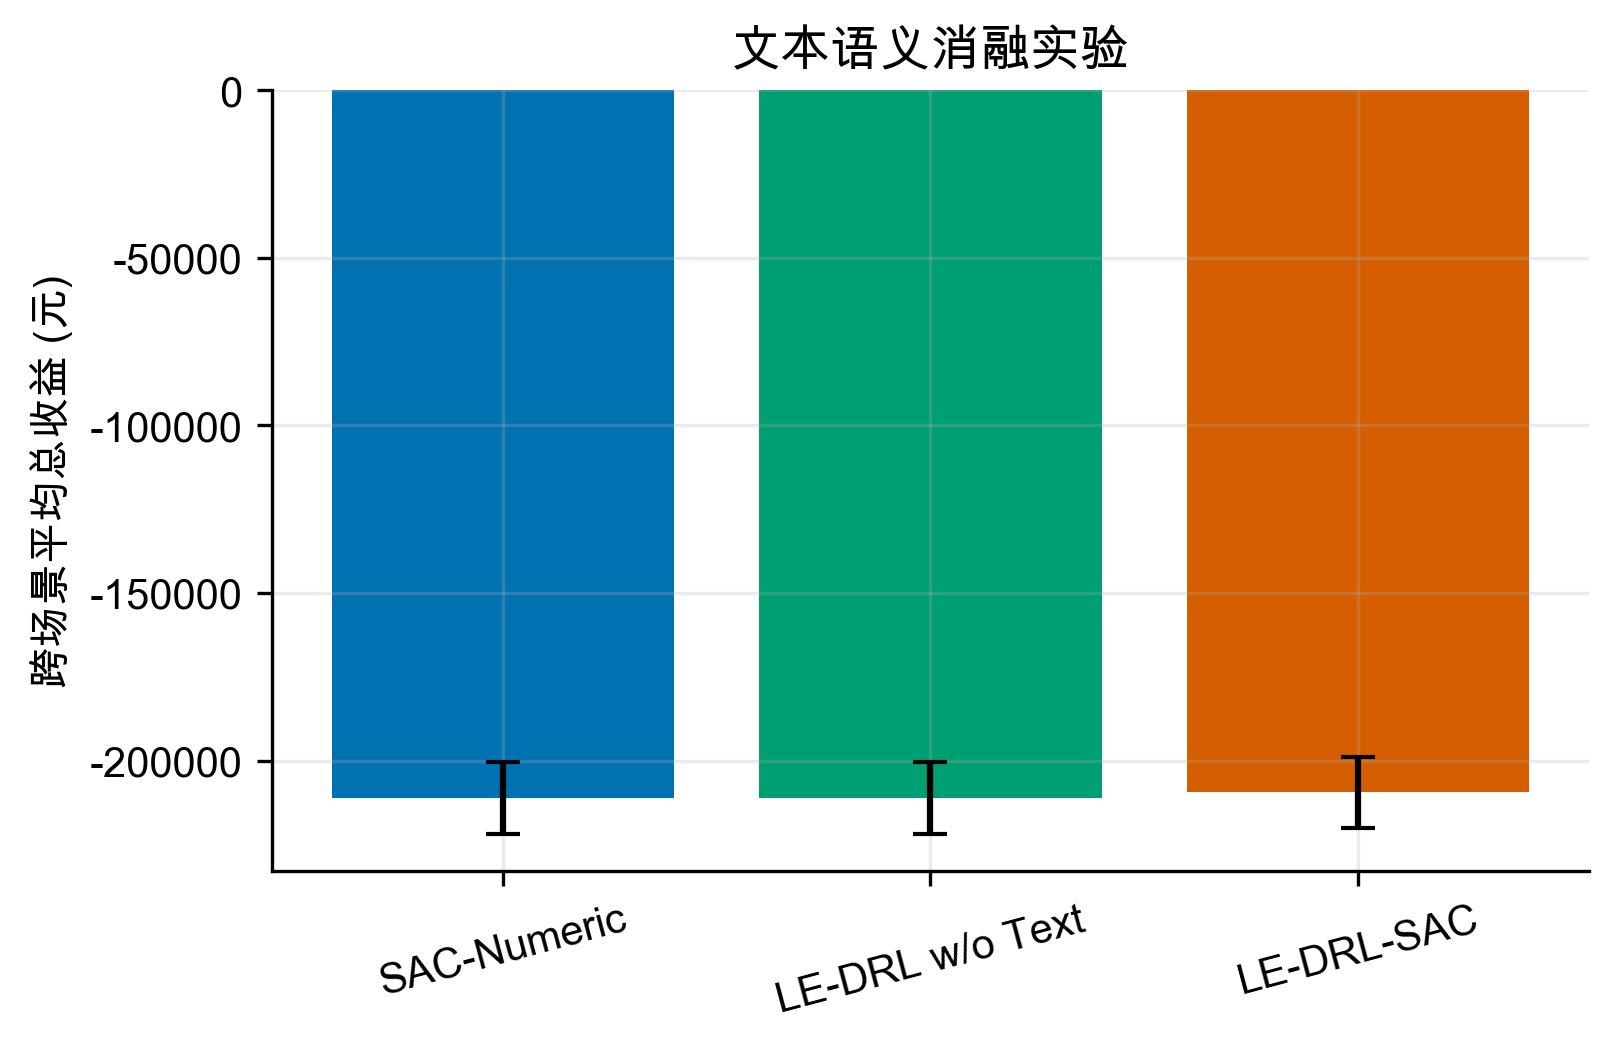
\includegraphics[width=0.98\columnwidth]{figures/text_ablation.png}
  \caption{Text-ablation comparison. The ablation model preserves the same input dimension but sets semantic features to zero.}
  \label{fig:text_ablation}
\end{figure}

Fig.~\ref{fig:s3_traj} shows the S3 price-spike SOC and action trajectories for the trained SAC variants. LE-DRL-SAC produces more active charging and discharging behavior than the numerical SAC and text-ablation baselines. The behavior is consistent with the semantic signal: price-spike events encourage high-price discharge, while low-price or renewable-absorption periods encourage charging.

\begin{figure}[t!]
  \centering
  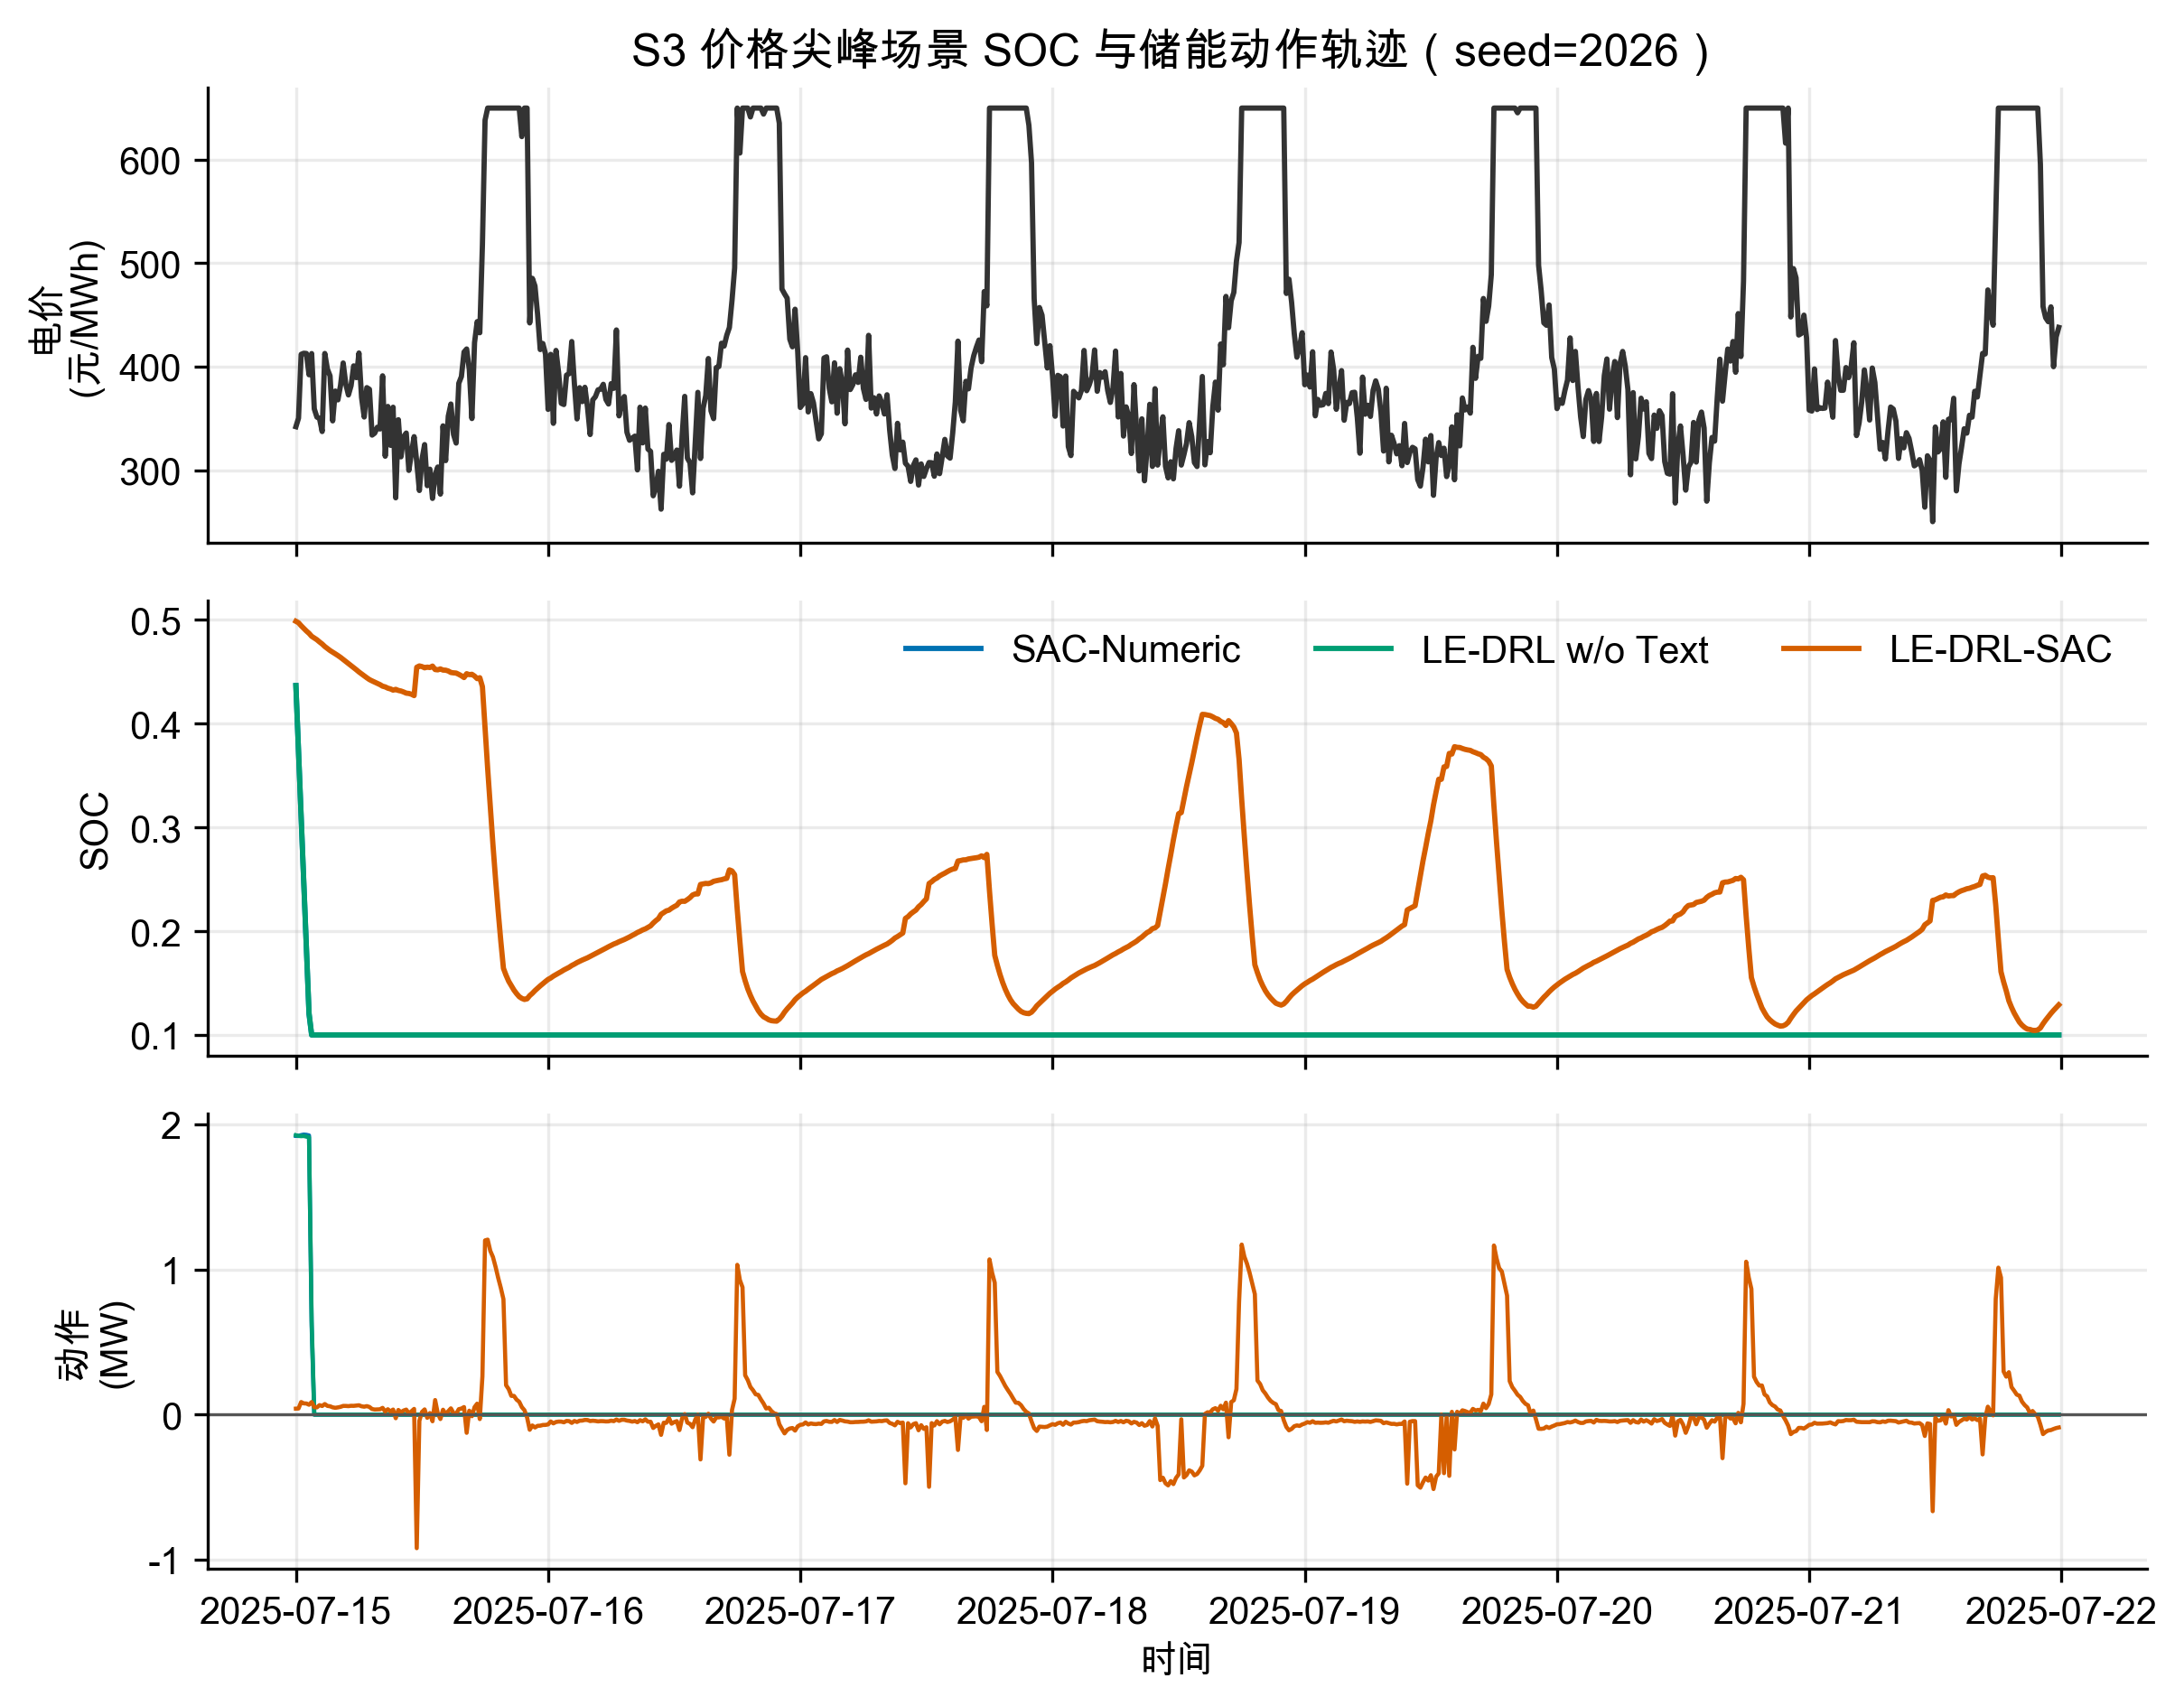
\includegraphics[width=0.98\columnwidth]{figures/s3_soc_action_trajectory.png}
  \caption{SOC and action trajectories in the price-spike scenario. LE-DRL-SAC learns more event-responsive battery behavior.}
  \label{fig:s3_traj}
\end{figure}

\subsection{Discussion}
The results support four conclusions. First, DeepSeek-derived semantic features provide measurable value over numerical SAC in the calibrated VPP dataset. Second, the text-ablation result shows that the gain is not merely caused by a larger input vector: SAC-Numeric and LE-DRL w/o Text remain nearly identical, whereas LE-DRL-SAC improves when nonzero semantic scores are supplied. Third, the learned actor alone is not sufficient to outperform strong operational baselines on the known-event scenarios; the semantic safety layer is necessary for the final controller to exceed the implemented Rule-Based, Rolling-Horizon, and Enhanced Rolling-Horizon baselines in average total reward. Fourth, the numeric safety layer ablation demonstrates that the safety-layer mechanism itself is useful but not sufficient: a purely numeric safety layer improves SAC-Numeric from -211,023.2 to -209,125.3 yuan, yet the language-enhanced semantic safety layer still reaches -208,468.9 yuan, so the residual improvement is attributable to structured text-derived semantic features rather than to the blending mechanism alone. The current evidence does not by itself prove that DeepSeek is uniquely superior to a simpler keyword or noisy semantic encoder, because that dedicated comparison is not yet reported. It supports the narrower claim that structured semantic features extracted from event text improve the dispatch controller relative to zero-text and numeric-prior ablations. To quantify uncertainty we use a seed-paired bootstrap: for each of the 12 matched (seed, scenario) pairs we form the reward difference proposed minus baseline and resample these paired differences 20{,}000 times with replacement, reporting the 2.5th--97.5th percentile of the bootstrap mean. This preserves the seed-matched pairing (the same seed is always compared against itself) and reflects scenario-level variability rather than only the three seed means. A two-sided Wilcoxon signed-rank test on the same paired differences is reported as a non-parametric cross-check. For the proposed controller versus SAC-Numeric the paired difference is $+2{,}554.2$ yuan with 95\% bootstrap CI $[+2{,}060.4, +3{,}043.8]$ and Wilcoxon $p=0.0005$, so the CI excludes zero by a wide margin. The earlier draft reported an implausibly narrow CI ($[+2{,}517.9, +2{,}573.6]$, width 55 yuan) obtained by resampling only three seed-level means; that interval reflected the near-zero seed variance of SAC-Numeric rather than the uncertainty of the reward difference and is replaced here by the paired-bootstrap interval. The main cross-scenario comparison uses three seeds; the new-event adaptation study in Section~\ref{sec:unseen_event} and the parameter-variant study use five seeds with the same paired-bootstrap procedure, yielding intervals such as $[+4{,}875, +6{,}074]$ on S5 and $[+3{,}549, +5{,}556]$ on V4 that corroborate the adaptation effect rather than a seed-level artifact.

A fifth conclusion, drawn from the new-event adaptation study, refines the picture. On the four known events the prior dominates and the learned actor contributes a bounded correction; on the newly introduced negative-price-surplus event the prior has no matching branch and the learned actor, freed from the semantic-consistency regularizer and allowed to learn from the LLM features during S1--S5 adaptation, takes over and exceeds text-agnostic SAC-Numeric by 5{,}482 yuan (95\% bootstrap CI [+4{,}875, +6{,}074], all five seeds favorable). The regularizer sweep reveals that the actor semantic-consistency regularizer plays two separable roles: on known events it stabilizes training without changing the final reward (within 0.5\% across weights), while on the new event a lower weight yields an 18{,}515-yuan improvement as the actor gains freedom to learn cross-interval SOC management. The regularizer is therefore retained for the known-event configuration and relaxed for the new-event adaptation configuration, with its two roles---a known-event stabilizer and an adaptation constraint---made explicit. Together, these results indicate that language-derived risk semantics play two separable roles---a state feature that the actor learns from, and a training target that constrains the actor---and that the optimal balance between a pre-designed prior and a learned actor is itself event-coverage-dependent. This is why the safety-layer weight is treated as an event-coverage-dependent quantity in this paper rather than a universal constant.

The safety-layer result should be interpreted carefully. It does not mean that an LLM directly solves VPP dispatch. The language module only produces structured risk features. The safety layer then maps these features into bounded and physically checked action corrections. This is closer to an event-aware supervisory control layer than to free-form language-model control. Such a design is more suitable for power-system applications because it keeps the final dispatch action deterministic, auditable, and constrained. The Enhanced Rolling-Horizon optimizer further demonstrates that aggressive short-horizon optimization can achieve competitive reward at the price of excessive battery cycling (133.16 MWh); engineering regularization reduces this to 14.80 MWh, which is more consistent with operational battery-life constraints.

Although the absolute total-reward gap between the proposed controller and the rule-based baseline appears modest in percentage terms (approximately 0.24\%), this is an inherent property of the reward structure rather than a weakness of the method: the bulk of the total reward originates from the unavoidable net-export revenue that any feasible policy accrues, so the marginal value of smarter battery control is small relative to the absolute reward. Three observations indicate that the improvement is nonetheless substantive. First, on tail risk the proposed controller improves CVaR 5\% from -705.0 yuan (Rule-Based) to -696.7 yuan, a 1.2\% reduction in worst-step losses, which is more operationally meaningful than the headline total-reward figure. Second, on behavioral indicators the proposed controller raises the high-price discharge rate from 0.176 (Rule-Based) to 0.231, a 31\% relative increase, showing that the policy concentrates discharging in high-price intervals rather than merely increasing total throughput. Third, the advantage is scenario-dependent and largest exactly where textual event semantics should matter most: in the price-spike scenario the proposed controller reaches -218,660.5 yuan versus -219,146.3 yuan for Rule-Based, and the out-of-distribution evaluation confirms that the event-driven scenarios (S2, S4) are where the language-enhanced policy consistently leads. We therefore report the total-reward gap alongside CVaR and behavioral metrics, and refrain from overstating the headline percentage.

The remaining limitation is data validity. The main cross-scenario trajectories are public-data-calibrated generated sequences rather than verified private VPP telemetry. This concern is addressed progressively along an increasing-realism ladder: the following subsection first replaces the weather-driven channels with real Guangzhou observations (Section~\ref{sec:ood}); the new-event adaptation study then replaces both the price series and the weather with real German DE-LU day-ahead prices and real Open-Meteo weather (Section~\ref{sec:unseen_event}, real-price validation). The DE-LU experiment is the point on this ladder closest to a real market, and the language-enhanced advantage persists there under genuine negative prices---which is the key evidence that the event-awareness mechanism named in the title is not an artifact of the synthetic generator. The next step for an even stronger submission is to validate the same method on measured private VPP or microgrid telemetry and to compare it with a full MILP/MPC rolling optimizer under identical forecasts and battery constraints.

\subsection{Out-of-Distribution Evaluation on Real Weather}
\label{sec:ood}
Because the training scenarios are synthetic 2025-07 sequences, a natural concern is whether the learned policy generalizes to data drawn from a different distribution. To examine this, an out-of-distribution (OOD) test set was constructed by retrieving real Guangzhou weather observations for July 2024 from the Open-Meteo Historical Weather API and resampling the hourly temperature and solar-radiation records to the 15-minute resolution. The temperature and PV-driving channels of the four event scenarios were then replaced by these real observations, whereas the load, price, and event-text channels were retained from the generator so that the reward and event semantics remain comparable with the training set. The OOD set therefore differs from the training distribution in year and in the weather-driven dynamics, while preserving the same scenario structure.

Table~\ref{tab:ood_summary} reports the cross-scenario averages. The proposed LE-DRL-SAC with semantic safety layer attains the highest average total reward (-211,307.4 yuan), exceeding the rule-based controller (-211,467.2 yuan), the SAC-Numeric with numeric safety layer (-211,425.2 yuan), the Enhanced Rolling-Horizon optimizer (-211,558.9 yuan), and the Rolling-Horizon optimizer (-211,699.2 yuan). At the scenario level, the proposed controller achieves the best total reward in OOD-S2 (high-temperature load pressure) and OOD-S4 (renewable-curtailment pressure), which are precisely the event-driven scenarios where textual risk semantics are expected to provide the most value. In OOD-S1 (normal operation), the proposed controller is marginally below the rule-based and numeric-safety-layer baselines, because the more active policy learned under event pressure induces slightly higher cycling on a benign trajectory; this is consistent with the throughput figures in Table~\ref{tab:ood_summary}. In OOD-S3 (price spike), the Rolling-Horizon optimizer remains strongest, consistent with the in-distribution result that short-horizon look-ahead is particularly effective under explicit price-spike dynamics. The learned policy continues to exhibit nonzero battery throughput and event-responsive behavior on the real-weather data. This result provides preliminary evidence that the proposed framework does not collapse when the weather-driven channels are replaced by real observations, with the advantage concentrated in event-driven scenarios; however, because load, price, and event-text channels were retained from the generator, this test should be interpreted as a distribution-shift check rather than a full OOD generalization claim. Validation on measured VPP telemetry remains necessary.

\begin{table}[t!]
\caption{OOD Cross-Scenario Summary on Real Guangzhou Weather (2024-07)}
\label{tab:ood_summary}
\centering
\begin{tabular}{lcc}
\toprule
\textbf{Model} & \textbf{Total reward (yuan)} $\uparrow$ & \textbf{Throughput (MWh)} \\
\midrule
LE-DRL-SAC + semantic safety layer & \textbf{-211,307.4} & 8.50 \\
SAC-Numeric + numeric safety layer & -211,425.2 & 4.44 \\
Rule-Based & -211,467.2 & 4.27 \\
Enhanced Rolling-Horizon & -211,558.9 & 10.50 \\
Rolling-Horizon & -211,699.2 & 134.03 \\
\bottomrule
\end{tabular}
\end{table}

\begin{figure}[t!]
  \centering
  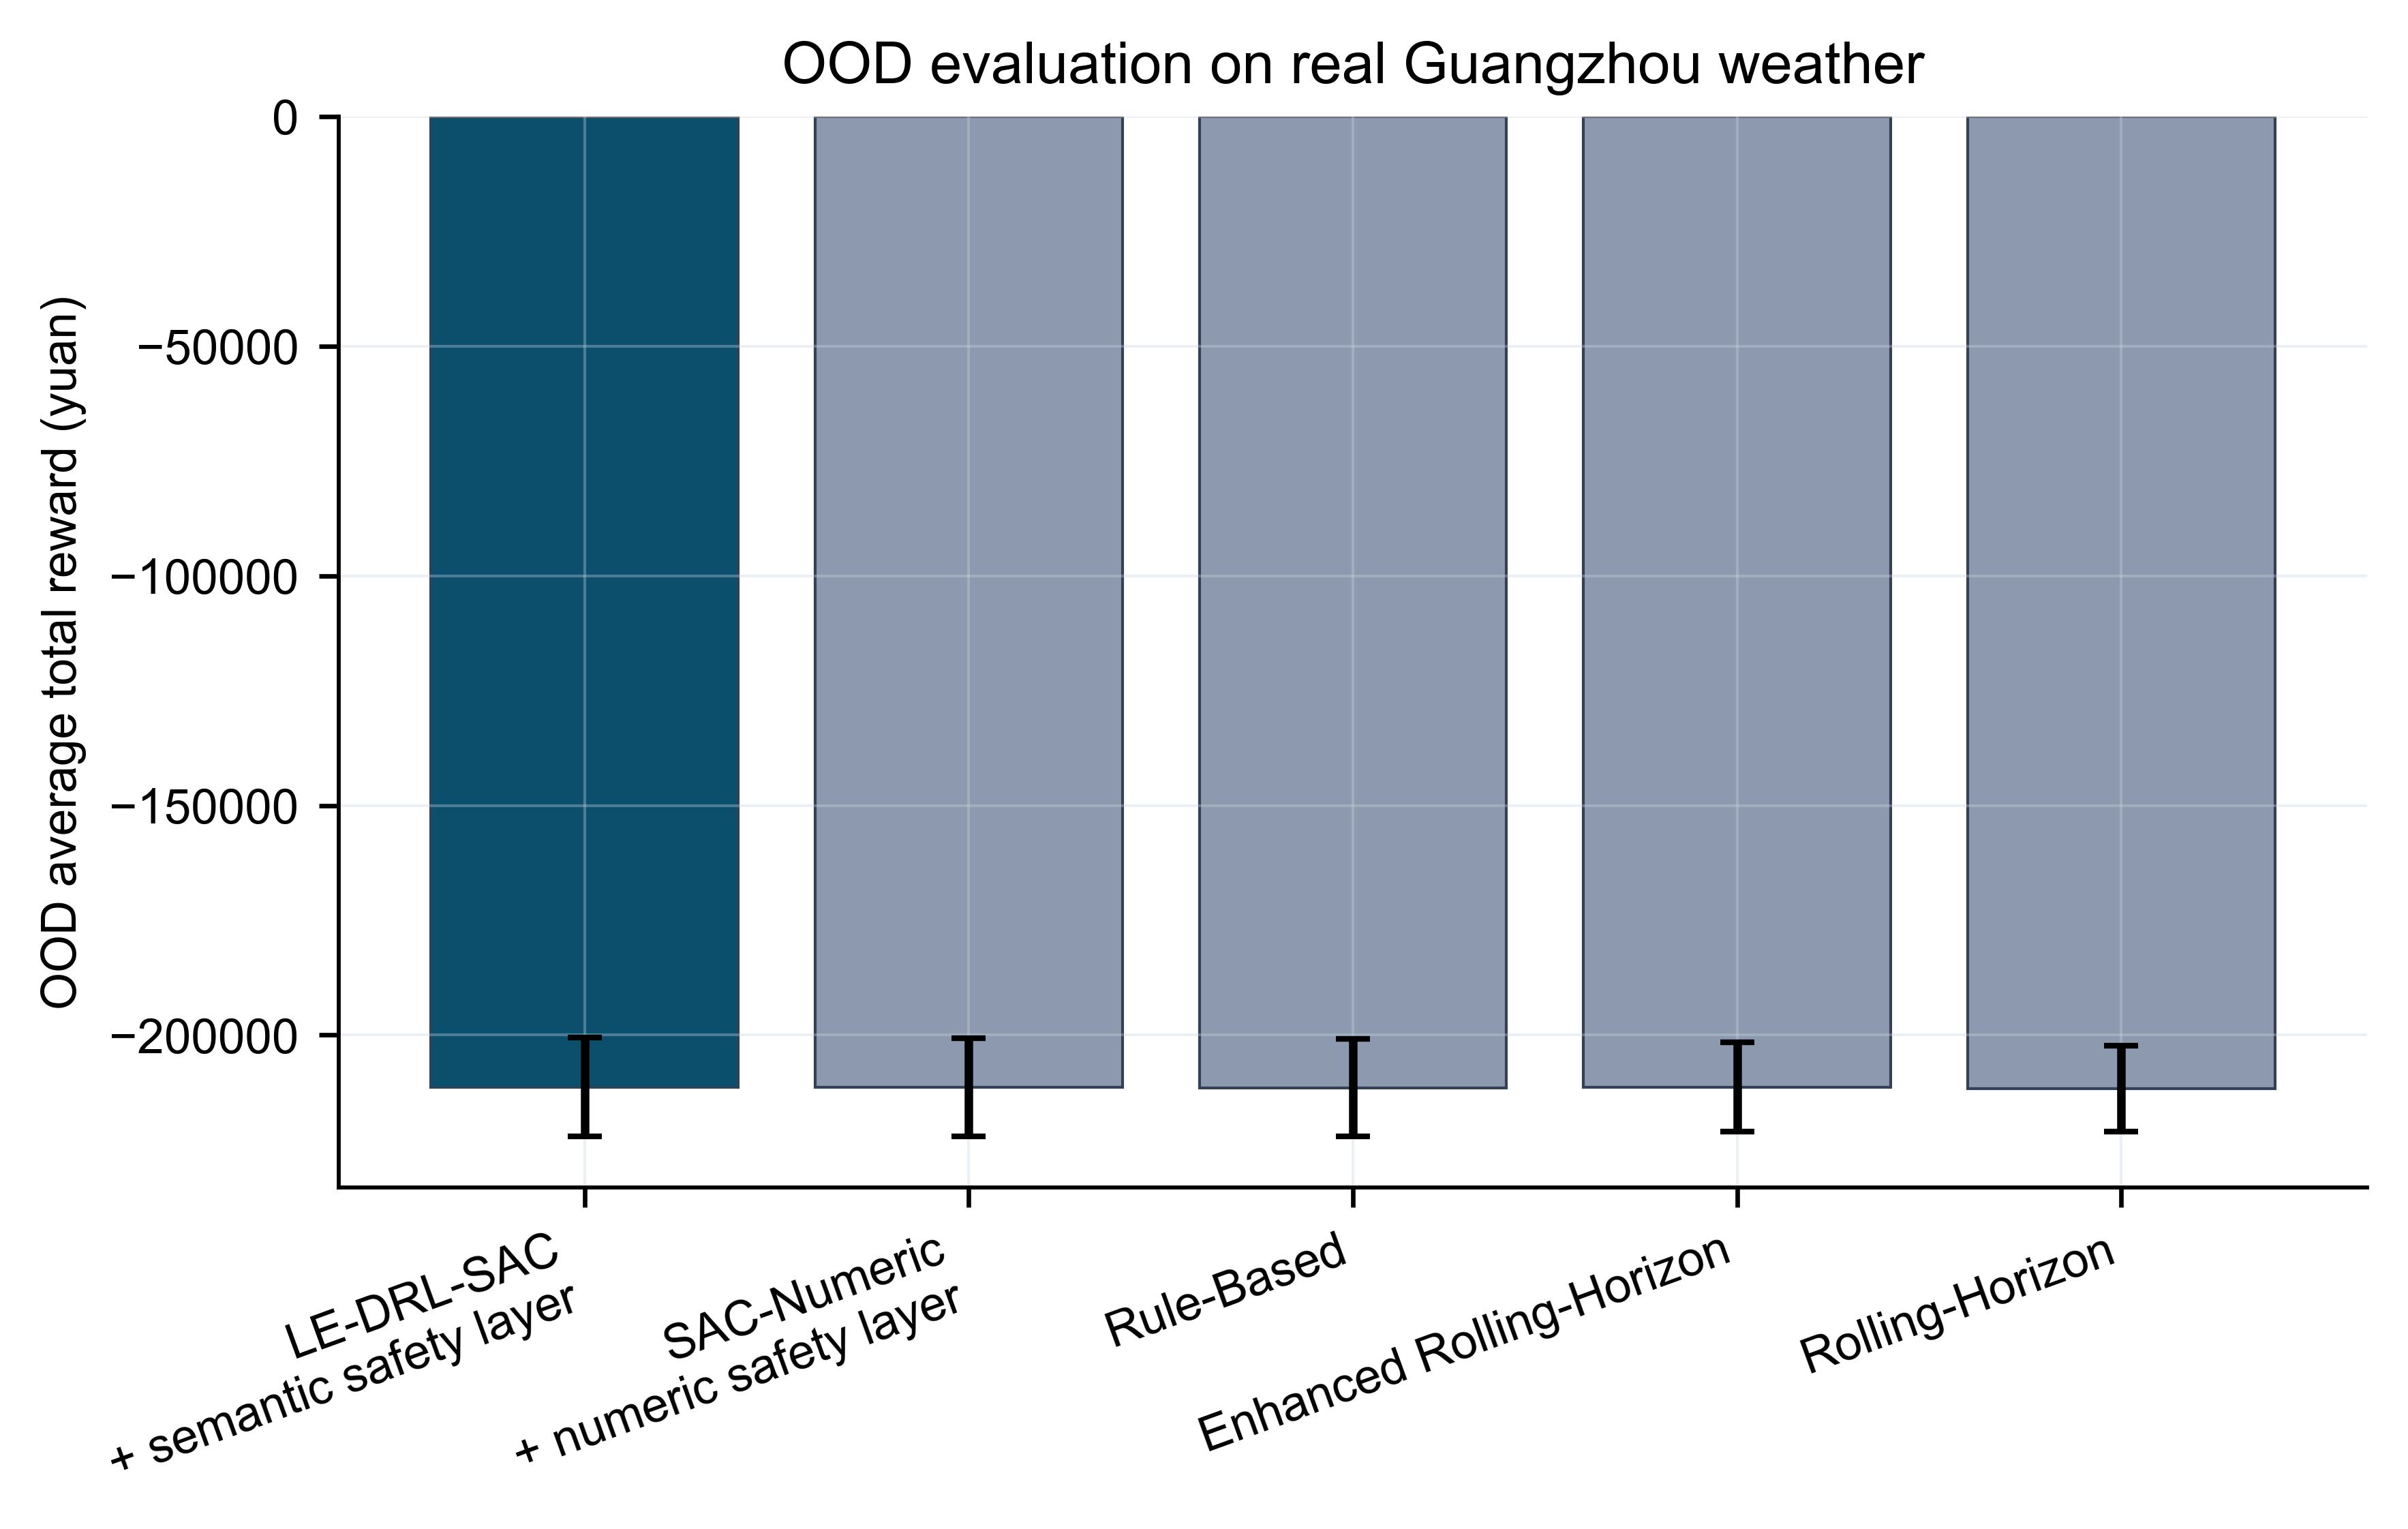
\includegraphics[width=0.98\columnwidth]{figures/ood_real_weather_reward.png}
  \caption{OOD cross-scenario average total reward on real Guangzhou weather observations (July 2024) with scenario variability. The proposed controller retains the highest average reward when the temperature and PV channels are replaced by real observations.}
  \label{fig:ood_reward}
\end{figure}

\subsection{Generalization to Unseen Event Expressions}
\label{sec:unseen_text}
A natural concern is whether the DeepSeek semantic encoder merely matches the five fixed training templates rather than responding to event meaning. To examine this, an unseen-expression test set was constructed in which each event category was rewritten into five paraphrases that differ in wording from the training template but preserve the operational meaning (for example, the high-temperature warning was paraphrased as ``南方区域持续高温，空调负荷预计在晚高峰快速攀升'' [``Sustained high temperature in the southern region; air-conditioning load is expected to rise rapidly toward the evening peak''] and ``气象部门提示未来数小时出现极端炎热天气'' [``The meteorological service indicates extreme heat in the coming hours'']). DeepSeek (\texttt{deepseek-chat}, accessed via an OpenAI-compatible chat-completions interface with \texttt{temperature=0.1} and a structured JSON output format) was queried for each unseen expression using the same system prompt as the training templates. Table~\ref{tab:semantic_scores} compares the mean scores across the five paraphrases per category against the original training template; the scores are consistent at the category level, with the key dimensions (load pressure for temperature and demand-response events, price-spike pressure for price events, and curtailment pressure for renewable events) deviating by at most $\pm0.1$. This result supports paraphrase-level robustness of the DeepSeek scores, but it is not a substitute for a keyword/noisy-score ablation.

\begin{table*}[t!]
\caption{DeepSeek Semantic Scores: Training Template vs. Unseen Paraphrases (Mean of Five)}
\label{tab:semantic_scores}
\centering
\begin{tabular}{lccccc}
\toprule
\textbf{Event category} & \textbf{Source} & \textbf{Load pressure} & \textbf{Price-spike} & \textbf{Curtailment} & \textbf{Storage bias} \\
\midrule
\multirow{2}{*}{High-temperature} & Template & 0.80 & 0.60 & 0.20 & -0.50 \\
& Unseen (mean of 5) & 0.86 & 0.78 & 0.12 & -0.58 \\
\multirow{2}{*}{Price spike} & Template & 0.60 & 0.80 & 0.30 & -0.50 \\
& Unseen (mean of 5) & 0.54 & 0.86 & 0.24 & -0.68 \\
\multirow{2}{*}{Demand response} & Template & 0.90 & 0.80 & 0.20 & -0.60 \\
& Unseen (mean of 5) & 0.84 & 0.70 & 0.22 & -0.54 \\
\multirow{2}{*}{Renewable curtailment} & Template & 0.40 & 0.20 & 0.80 & 0.70 \\
& Unseen (mean of 5) & 0.34 & 0.18 & 0.80 & 0.66 \\
\bottomrule
\end{tabular}
\end{table*}


The proposed controller was then re-evaluated on the unseen-text scenarios, which reuse the real-weather OOD trajectories but replace the event text with the unseen paraphrases. The proposed controller attains the highest cross-scenario average total reward (-211,314.7 yuan), exceeding the rule-based controller (-211,467.2 yuan) and the numeric-safety-layer SAC (-211,425.2 yuan), and the result is within 7 yuan of the original-template OOD reward (-211,307.4 yuan). At the scenario level, the proposed controller leads in the high-temperature load-pressure (S2) and renewable-curtailment (S4) scenarios, which are precisely the event-driven settings where textual semantics should matter. The near-identical reward under unseen wording indicates that the policy is not sensitive to the specific surface templates tested here; stronger evidence against keyword matching would require an explicit keyword-encoder and noisy-score baseline.

\subsection{New-Event Adaptation Study}
\label{sec:unseen_event}
The unseen-text test in Section~\ref{sec:unseen_text} reuses the four training event categories with paraphrased wording. A stronger adaptation question is whether the framework can respond after a new event \emph{category} is introduced outside the initial S1--S4 training set and outside the hand-crafted prior design. The hand-crafted semantic safety prior in Section~\ref{sec:method} was designed with four event branches keyed to known price thresholds, PV surplus, and the evening peak; it has no branch for negative prices, which arise in high-renewable-penetration markets when midday PV surplus collapses the spot price below zero. Such an event exposes a structural limitation of a pre-designed prior: it cannot be extended to a new category without rewriting its branches, whereas a learning actor can be retrained on the new event's cached semantic scores. This subsection therefore evaluates adaptation after S5 is added to the training set, not zero-shot generalization to an event never observed by the actor and not direct LLM control.

\textbf{Scenario S5: negative-price deep surplus.} A fifth seven-day scenario (S5) is generated by the same data generator as S1--S4 but with a negative-price stress transform: midday PV is boosted toward the plant ceiling during 10:00--15:00 and the spot price is driven below zero by a smooth dip centered at 12:30, while the evening-peak price is depressed rather than spiked. On S5, 96 of 672 steps clear at negative price (midday minimum $-210.4$ yuan/MWh), the evening peak averages 280.2 yuan/MWh with no spike, and midday PV averages 3.88~MW against 3.91~MW load. The correct response is to charge aggressively during the negative-price window to absorb PV surplus, to stop once the battery is full, and to discharge during the genuinely high-price intervals (which on S5 fall in the early morning rather than the evening). The prior's evening-peak discharge branch, which assumes ``evening peak = high price,'' is therefore misaligned with S5. The DeepSeek semantic encoder is queried once for the new event text; it returns renewable-curtailment pressure 0.90 and storage-bias $+0.80$, confirming that the LLM recognizes the surplus nature of the event even though the prior has no matching branch.

\textbf{Relaxed-regularizer LE-DRL-SAC.} On the known-event scenarios the actor semantic-consistency regularizer stabilizes training but, as shown below, it also constrains the actor to imitate the semantic target mapping and suppresses cross-interval SOC management. To let the actor exploit the LLM features freely on the new event, a relaxed-regularizer variant is trained in which the regularizer weight is set to zero; the LLM-derived features still enter the state, the semantic auxiliary reward still provides a denser learning signal, and the semantic safety layer remains available but is deactivated ($w=0$) so that the final action is produced by the learned actor. The actor is trained on S1--S5 (five seeds, 80 episodes) so that it is exposed to the new category during adaptation, mirroring a deployment in which a new event type appears in operation and the actor is retrained on its cached semantic scores while the prior is left unchanged. Thus the comparison isolates the value of making the new event semantically observable to SAC; it does not replace SAC decisions with LLM decisions.

Table~\ref{tab:s5_unseen} reports the S5 results. The relaxed-regularizer LE-DRL-SAC attains $-141{,}068.4$ yuan, exceeding SAC-Numeric (retrained on the same S1--S5 set) at $-146{,}550.2$ yuan by 5{,}481.7 yuan. The 95\% confidence interval $[+4{,}875.3, +6{,}074.0]$ yuan is computed by paired bootstrap over the five matched seed-level reward differences (LE-DRL-SAC minus SAC-Numeric), using the same paired-difference procedure as the main comparison; all five seeds favor the language-enhanced policy. The behavioral indicators confirm that the gain stems from event-adaptive behavior: the relaxed LE-DRL-SAC charges during 100\% of the negative-price steps (versus 98\% for SAC-Numeric) while keeping the evening discharge near zero, i.e., it learns to avoid the prior's evening-peak discharge on a day when the evening price is depressed. The rule-based and full-regularizer rows are retained to show why the fixed prior is insufficient on this category, but the central statistical comparison is between two retrained SAC actors with and without LLM-derived semantic features.

\begin{table}[t!]
\caption{New-Event Adaptation on S5 (Negative-Price Surplus), Five Seeds}
\label{tab:s5_unseen}
\centering
\begin{tabular}{lcc}
\toprule
\textbf{Model} & \textbf{Total reward (yuan)} $\uparrow$ & \textbf{Neg-price charge rate} \\
\midrule
LE-DRL-SAC, relaxed regularizer, $w=0$ & \textbf{-141,068.4} & 0.99 \\
SAC-Numeric (retrained on S1--S5) & -146,550.2 & 0.99 \\
LE-DRL-SAC, full regularizer, $w=0$ & -159,670.6 & 0.08 \\
LE-DRL-SAC + safety layer ($w=0.9$, full reg.) & -161,009.4 & 0.00 \\
Rule-Based & -157,205.3 & 0.00 \\
\bottomrule
\end{tabular}
\end{table}

\textbf{Regularizer sensitivity.} Table~\ref{tab:actor_loss_sweep} sweeps the actor semantic-consistency regularizer weight on the S1--S5 training set (three seeds). On the four known-event scenarios the reward is essentially flat across regularizer weights (within 0.5\%), confirming that the regularizer is not a load-bearing component on known events. On S5, however, the reward improves monotonically as the regularizer is relaxed: from $-159{,}670.6$ yuan at the full weight to $-141{,}155.6$ yuan at zero weight, a gain of 18{,}515.0 yuan. The known-event rewards do not degrade under this relaxation. The five-seed relaxed-regularizer result in Table~\ref{tab:s5_unseen} ($-141{,}068.4$ yuan) corroborates the zero-weight row and confirms the gain under independent seeds. This indicates that the regularizer plays two distinct roles that conflict on newly introduced events: it aligns the actor with the semantic target on known categories, but the same alignment prevents the actor from learning the cross-interval SOC management that the negative-price event requires.

\begin{table}[t!]
\caption{Actor Semantic-Consistency Regularizer Sweep (Three-Seed Mean)}
\label{tab:actor_loss_sweep}
\centering
\begin{tabular}{lcccccc}
\toprule
\textbf{Weight} & \textbf{S1} & \textbf{S2} & \textbf{S3} & \textbf{S4} & \textbf{S5} & \textbf{Avg} \\
\midrule
0.0 & -203,502 & -220,255 & -222,024 & -198,307 & \textbf{-141,156} & -197,049 \\
0.5 & -203,534 & -220,291 & -222,053 & -198,343 & -146,983 & -198,241 \\
1.5 & -203,355 & -220,081 & -221,805 & -198,014 & -158,898 & -200,431 \\
3.0 & -203,120 & -219,892 & -220,896 & -197,735 & -159,671 & -200,263 \\
\bottomrule
\end{tabular}
\end{table}

\textbf{Interpretation.} Two conclusions follow. First, LLM-derived semantic features, consumed as state by a learning actor that is free to learn from them, let the policy adapt after a new event category is introduced and the hand-crafted prior cannot cover it; to our knowledge this provides preliminary evidence of such adaptation in LLM-enhanced dispatch, which future work on measured operational data should confirm. The result should be read as evidence for semantic-feature-assisted SAC adaptation, not as evidence that an LLM policy is superior to conventional control rules. Second, the result sharpens the event-coverage principle that motivates the safety-layer design: on known events the prior dominates and a strong regularizer is harmless, but on newly introduced events the learned actor must take over and a strong regularizer is harmful. This is why the safety-layer weight is treated as event-coverage-dependent in this paper: a single fixed weight cannot be optimal across both regimes. Automating the coverage-dependent weight selection is left to future work; the present paper establishes the principle with two fixed configurations (high weight on known events, zero weight with relaxed regularizer during new-event adaptation) and reports the trade-off explicitly.

\textbf{Parameter-variant robustness.} A natural concern is that S5 is a single hand-picked scenario. To address this, four structurally distinct negative-price variants were constructed that all satisfy the two headroom conditions (a deep negative-price window plus the absence of a high-price export opportunity) but vary across three independent dimensions: negative-price depth (V1 baseline vs.\ V2 deeper), season (V1 summer vs.\ V3 winter with weak PV and low load), and PV plant capacity (V1 5~MW vs.\ V4 4~MW, which changes the surplus-to-load ratio while preserving the midday-PV-surplus structure). The LE-DRL-SAC actor (relaxed regularizer, $w=0$) and SAC-Numeric were both retrained on S1--S5 and evaluated on the four held-out variants; the results are reported as mean pairwise reward gaps over five seeds with 95\% bootstrap confidence intervals.

\begin{table}[t!]
\caption{Unseen-Event Parameter Variants: LE-DRL-SAC minus SAC-Numeric (Five Seeds)}
\label{tab:s5_variants}
\centering
\begin{tabular}{lccc}
\toprule
\textbf{Variant} & \textbf{Gap (yuan)} & \textbf{95\% CI} & \textbf{Seeds favorable} \\
\midrule
V1 (S5-ref, noon, summer) & \textbf{+4,412} & [+3,303, +5,769] & 5/5 \\
V2 (deep, noon, summer) & +965 & [-5, +1,936] & 4/5 \\
V3 (noon, winter, weak PV) & \textbf{+5,001} & [+4,303, +5,725] & 5/5 \\
V4 (noon, summer, 4 MW PV) & \textbf{+4,407} & [+3,549, +5,556] & 5/5 \\
\bottomrule
\end{tabular}
\end{table}

The adaptation is robust across all three dimensions: V1, V3, and V4, which differ in PV capacity, season, and PV strength, all yield significant positive gaps (95\% CIs entirely above zero, all five seeds favorable), and V2 (deeper negative price) trends positive. The consistency across depth, season, and plant capacity indicates that the new-event adaptation is not an artifact of a single parameter setting; the language-enhanced policy consistently exceeds text-agnostic SAC when the held-out variant preserves the adapted event's surplus structure. This robustness motivates the learned gate in Section~\ref{sec:gated_moe}, which automates the coverage-dependent weight.

\textbf{Real-price validation.} To confirm that the negative-price event structure is not a synthetic artifact, a validation scenario was constructed from real German DE-LU day-ahead prices (SMARD/Bundesnetzagentur, CC BY 4.0, 2025-06-15 to 2025-07-05, hourly resolution interpolated to 15-minute, 21 consecutive days including workdays and weekends) and real Open-Meteo weather observations for the same location and period (shortwave radiation, temperature, and cloud cover resampled to 15 minutes). Unlike a single-day-tiled scenario, this three-week series exhibits genuine inter-day heterogeneity (consecutive-day price correlation 0.88, ranging from 0.63 to 0.98, with 14 of 21 days containing negative-price intervals and a minimum of $-99.0$~EUR/MWh), so the bootstrap confidence interval reflects independent daily patterns rather than a repeated template. The negative-price event text is planted only on intervals where the real price is negative, aligning the textual event with the real negative-price window, and the LLM semantic encoder is queried once for this event text. Because this scenario is priced in EUR/MWh, its rewards are reported in EUR (see the currency note in Section~\ref{sec:data}). On five seeds, the relaxed-regularizer LE-DRL-SAC attains a gap of $+$6{,}035~EUR over SAC-Numeric with a paired-bootstrap 95\% CI $[+5{,}415, +6{,}656]$ computed from the five matched seed-level reward differences; 5/5 seeds are favorable (Table~\ref{tab:real_price}). The gain is attributable to the LLM-derived semantic scores steering the actor toward charging during the real negative-price window and avoiding discharge during the depressed evening hours, a behavior that text-agnostic SAC learns more slowly from price alone. This validates that the new-event adaptation transfers to real negative-price records and real weather, not only to the calibrated S5 structure.

\begin{table}[t!]
\caption{Real-Price Validation on Multi-Week DE-LU Day-Ahead Prices (2025-06-15 to 2025-07-05), Reward Gap in EUR (Five Seeds)}
\label{tab:real_price}
\centering
\begin{tabular}{lccc}
\toprule
\textbf{Scenario} & \textbf{Gap (EUR)} & \textbf{95\% CI (EUR)} & \textbf{Seeds favorable} \\
\midrule
Real DE-LU price + real weather (3-week) & \textbf{+6{,}035} & [+5{,}415, +6{,}656] & 5/5 \\
\bottomrule
\end{tabular}
\end{table}

\subsection{Semantic-Source Ablation: Does the Actor Read LLM Semantics?}
\label{sec:m5_ablation}
A reviewer-relevant question is whether the gain of LE-DRL-SAC over SAC-Numeric is attributable to the actor genuinely reading the LLM-derived semantic features from the augmented state, or to indirect effects such as a larger input vector or a denser training reward. We isolate these mechanisms with three diagnostic baselines and three semantic sources under the main configuration ($w=0.9$, $\lambda_{\mathrm{sem}}=3.0$, S1--S4, five seeds).

\textbf{Three baselines.} (i) \emph{LE-DRL-SAC} (native): the actor reads the real semantic vector $s^{\mathrm{sem}}_t$ in $s^{\mathrm{aug}}_t$, and the semantic-consistency regularizer (Eq.~6) actively pulls the actor toward a semantic prior action. (ii) \emph{LE-DRL w/o Text}: the same 12-dim input is kept, but the five semantic dims are clamped to zero; the regularizer still fires but its target degenerates to a text-free prior. This isolates the value of the semantic \emph{content} from the value of the larger input vector. (iii) \emph{SAC-Numeric}: a 7-dim input with no semantic channel at all, isolating the value of the channel itself.

\textbf{Three semantic sources.} The $s^{\mathrm{sem}}_t$ fed to (i) and (ii) is drawn from one of: (a) DeepSeek (the main-paper source), (b) a local keyword encoder (\texttt{LocalSemanticEncoder}, a deterministic Chinese-keyword scorer), or (c) the DeepSeek scores perturbed by clipped Gaussian noise ($\sigma{=}0.20$ on risk dims, $\sigma{=}0.30$ on storage bias). Source (b) tests whether the gain is unique to LLM understanding or matched by structured text features; source (c) tests whether the semantic \emph{content} rather than the dimensionality carries the value.

\textbf{Result 1 --- the actor reads the semantic state.} Table~\ref{tab:m5_ablation} shows that under the main configuration LE-DRL-SAC (native) outperforms LE-DRL w/o Text on every known-event scenario under the DeepSeek source: S1 $+491.7$ yuan (95\% CI $[+433.5, +535.2]$, 5/5 seeds), S2 $+492.5$ ($[+480.0, +505.4]$, 5/5), S3 $+960.6$ ($[+910.4, +997.3]$, 5/5), and S4 $+1{,}224.7$ ($[+1{,}158.5, +1{,}261.0]$, 5/5). Pooled across the 20 matched (seed, scenario) pairs the gap is $+792.4$ yuan (95\% CI $[+654.7, +934.0]$, 20/20 favorable). Because the two baselines share the same 12-dim input and the same regularizer activation, the only difference is whether the semantic dims carry real scores or are zeroed. The consistent, all-seed-favorable advantage of native therefore cannot be attributed to input-dimension expansion and confirms that the SAC actor, under the semantic-consistency regularizer, learns to read the LLM-derived features in $s^{\mathrm{sem}}_t$ and act on them. This is the direct evidence for the language-enhanced mechanism named in the title. The advantage is scenario-dependent and largest exactly where textual semantics should matter most---S4 renewable-curtailment ($+1{,}225$) and S3 price-spike ($+961$)---consistent with the main-paper observation in Section~\ref{sec:results}.

\textbf{Result 2 --- the semantic content matters, not just the dimensionality.} The noisy-source variant perturbs the DeepSeek scores with clipped Gaussian noise while keeping the same five dims active. Under noise, LE-DRL-SAC reward falls \emph{below} the zeroed-semantics baseline: the pooled native-minus-w/o-Text gap reverses to $-1{,}429.1$ yuan (95\% CI $[-2{,}170.5, -548.5]$, 5/20 favorable). In other words, semantic dims carrying \emph{wrong} values are worse than semantic dims carrying \emph{no} values: the actor, having been trained by the semantic-consistency regularizer to trust the semantic channel, is misled when that channel is corrupted. This confirms that the actor exploits the semantic \emph{values}, not merely the presence of the channel. The DeepSeek-minus-noisy pooled gap is $+2{,}221.5$ yuan (95\% CI $[+1{,}382.7, +2{,}945.0]$, 15/20), reinforcing that genuine semantic content is load-bearing.

\textbf{Result 3 --- DeepSeek vs.\ keyword encoder on known events.} The local keyword encoder (\texttt{LocalSemanticEncoder}) is a deterministic Chinese-keyword scorer hand-designed for the four known event categories. Under the main configuration it performs comparably to DeepSeek: the pooled native gap (DeepSeek minus keyword) is $-28.4$ yuan (95\% CI $[-63.6, +8.3]$, 6/20 favorable), statistically indistinguishable from zero. This indicates that for the four \emph{known} event categories, which the keyword encoder was designed to cover, structured text-derived scores are sufficient and the LLM offers no distinct advantage. The LLM's distinct value is exposed precisely outside that coverage, as shown in Result~4.

\textbf{Result 4 --- Zero-maintenance generalization to an event category outside the keyword table (S8).} Results 1--3 establish that on the four known event categories, which the keyword table was hand-designed to cover, the DeepSeek and keyword sources are statistically indistinguishable: structured text-derived scores are sufficient there and the LLM confers no distinct advantage. The complementary question is what happens when an event category arises that the deployed encoder was \emph{not} configured for. We therefore construct S8, a frequency-reserve request in which the correct response (keep SOC mid-band for bidirectional reserve) opposes the physical signal (PV surplus $\to$ charge $\to$ fill up), the reserve intervals are scattered across all hours so the numeric hour-of-day feature cannot predict them, and a reserve-capacity penalty $\rho(\mathrm{SOC}-0.5)^2$ ($\rho=600$) applies only during intervals whose event text signals a reserve request. Under the main configuration, LE-DRL-SAC with DeepSeek features attains $-203{,}876.1$ yuan against $-204{,}664.7$ yuan for the keyword encoder, a gap of $+788.6$ yuan (95\% CI $[+743.3, +837.5]$, 5/5 seeds favorable) with a lower reserve penalty ($1{,}803.7$ vs.\ $2{,}337.5$ yuan); SAC-Numeric, which has no event-text channel, pays the highest penalty ($3{,}746.4$) and keeps mid-band on only $2.5\%$ of reserve steps.

The mechanism behind the gap is not that the LLM ``understands'' better in the abstract, but that it generalizes to the new category with \emph{zero configuration}: the deployed keyword table has no frequency/reserve branch, so it returns all-zero scores and cannot steer the actor away from filling up, whereas the same cached DeepSeek query recognizes the reserve request and returns curtailment $0.20$ and storage-bias $0.0$ (no charge bias, keep mid-band). A keyword table extended with a hand-written reserve branch would in principle recover much of this gap---exactly as it does on S1--S4---but only after an engineer anticipates the category and rewrites the table. This is the operationally relevant distinction for a deployed VPP: event categories evolve, and a rule-based encoder must be manually extended for each new one, whereas the LLM encoder supplies a usable semantic vector for a previously undefined event category without any table maintenance. S8 is thus best read not as evidence that the LLM is intrinsically smarter, but as a concrete instance of the event-coverage principle at the encoder level: the LLM's value is exposed precisely outside the coverage that a hand-crafted component was built for.

\begin{table}[t!]
\caption{Semantic-Source Ablation on S1--S4, Main Config ($w=0.9$, $\lambda_{\mathrm{sem}}=3.0$), Five-Seed Mean Reward (yuan)}
\label{tab:m5_ablation}
\centering
\begin{tabular}{llrrrr}
\toprule
\textbf{Source} & \textbf{Model} & \textbf{S1} & \textbf{S2} & \textbf{S3} & \textbf{S4} \\
\midrule
\multirow{3}{*}{DeepSeek} & LE-DRL-SAC (native) & -88,561.1 & -94,903.9 & -95,553.3 & -85,422.1 \\
 & LE-DRL w/o Text & -89,052.7 & -95,396.4 & -96,513.9 & -86,646.8 \\
 & SAC-Numeric & -89,052.9 & -95,397.0 & -96,514.3 & -86,647.2 \\
\midrule
\multirow{3}{*}{Keyword} & LE-DRL-SAC (native) & -88,532.3 & -94,787.9 & -95,565.9 & -85,440.6 \\
 & LE-DRL w/o Text & -89,052.7 & -95,396.4 & -96,513.9 & -86,646.8 \\
 & SAC-Numeric & -89,052.9 & -95,397.0 & -96,514.3 & -86,647.2 \\
\midrule
\multirow{3}{*}{Noisy} & LE-DRL-SAC (native) & -91,552.6 & -98,157.9 & -94,666.3 & -88,949.3 \\
 & LE-DRL w/o Text & -89,052.7 & -95,396.4 & -96,513.9 & -86,646.8 \\
 & SAC-Numeric & -89,052.9 & -95,397.0 & -96,514.3 & -86,647.2 \\
\bottomrule
\end{tabular}
\end{table}

\begin{table}[t!]
\caption{Native (LE-DRL-SAC) minus w/o-Text gap, pooled over 20 (seed, scenario) pairs, 95\% paired-bootstrap CI}
\label{tab:m5_gaps}
\centering
\begin{tabular}{lrrr}
\toprule
\textbf{Semantic source} & \textbf{Gap (yuan)} & \textbf{95\% CI} & \textbf{Favorable} \\
\midrule
DeepSeek & \textbf{+792.4} & $[+654.7, +934.0]$ & 20/20 \\
Keyword & \textbf{+820.8} & $[+700.2, +946.7]$ & 20/20 \\
Noisy ($\sigma{=}0.20$) & -1,429.1 & $[-2{,}170.5, -548.5]$ & 5/20 \\
\bottomrule
\end{tabular}
\end{table}

\begin{table}[t!]
\caption{S8 Frequency-Reserve Event Outside the Keyword Table, Main Config ($w=0.9$, $\lambda_{\mathrm{sem}}=3.0$, $\rho=600$), Five-Seed Mean}
\label{tab:m5_s8}
\centering
\begin{tabular}{llrrr}
\toprule
\textbf{Source} & \textbf{Model} & \textbf{Reward} & \textbf{Reserve cost} & \textbf{Mid-band rate} \\
\midrule
DeepSeek & LE-DRL-SAC & \textbf{-203,876.1} & \textbf{1,803.7} & 0.225 \\
Keyword & LE-DRL-SAC & -204,664.7 & 2,337.5 & 0.225 \\
DeepSeek & SAC-Numeric & -207,512.1 & 3,746.4 & 0.025 \\
\bottomrule
\end{tabular}
\end{table}

\subsection{Learned Event-Coverage Gate}
\label{sec:gated_moe}
The two fixed configurations in the preceding subsections---high $w$ on known events and $w=0$ with a relaxed regularizer during new-event adaptation---instantiate the event-coverage principle but require the coverage label to be known at deployment time. This subsection examines whether the label can itself be learned from data. A gated mixture-of-experts controller is constructed: two SAC experts share the same LLM-augmented state but differ in regularization---a \emph{prior} expert with the semantic-consistency regularizer (strong on known events) and a \emph{free} expert without it (adaptive on new or held-out negative-price events)---and a small gate network $g_\psi(s)$ maps the encoded state to a blend weight $w\in[0,1]$ so that the final action is $a=(1-w)\,a^{\mathrm{free}}+w\,a^{\mathrm{prior}}$. The gate is trained by binary cross-entropy on a per-batch-normalized $Q$-difference target: for each state, the target is $1$ (favor the prior expert) where the prior expert's critic reports a higher $Q$ than the free expert's, and $0$ otherwise. Per-batch normalization removes the shared scale bias between the two critics so that the gate learns only the state-relative ordering, not a global offset.

The gate-training procedure is summarized in Algorithm~\ref{alg:gate}. The two SAC experts are trained first; the gate is then fitted on a held-out batch by binary cross-entropy on the per-batch-normalized $Q$-difference target, so that no event-coverage label is supplied.

\begin{algorithm}[t!]
\caption{Learned Event-Coverage Gate Training}
\label{alg:gate}
\begin{algorithmic}[1]
\Require LLM-augmented state $s^{\mathrm{aug}}$, replay batch $\mathcal{B} \subset \mathcal{D}$
\Require trained prior expert $\pi^{\mathrm{prior}}_\theta, Q^{\mathrm{prior}}_\phi$; trained free expert $\pi^{\mathrm{free}}_\theta, Q^{\mathrm{free}}_\phi$
\Require gate network $g_\psi$ (outputs $w \in [0,1]$)
\State \textbf{// Stage 1: pre-train the two SAC experts (Algorithm~\ref{alg:ledrl} Stage 2)}
\State train $\pi^{\mathrm{prior}}_\theta$ \textbf{with} the semantic-consistency regularizer ($\lambda_{\mathrm{sem}}>0$)
\State train $\pi^{\mathrm{free}}_\theta$ \textbf{without} the regularizer ($\lambda_{\mathrm{sem}}=0$)
\State \textbf{// Stage 2: build per-batch-normalized Q-difference targets}
\State sample batch $\mathcal{B} = \{s^{\mathrm{aug}}_i, a_i\}_{i=1}^{N}$
\State $q^{\mathrm{prior}}_i \gets Q^{\mathrm{prior}}_\phi(s^{\mathrm{aug}}_i, a_i)$,\quad $q^{\mathrm{free}}_i \gets Q^{\mathrm{free}}_\phi(s^{\mathrm{aug}}_i, a_i)$
\State $\tilde{q}^{\mathrm{prior}} \gets (q^{\mathrm{prior}} - \mu)/\sigma$,\quad $\tilde{q}^{\mathrm{free}} \gets (q^{\mathrm{free}} - \mu)/\sigma$ \Comment{per-batch normalization}
\State $y_i \gets \mathbb{1}[\tilde{q}^{\mathrm{prior}}_i > \tilde{q}^{\mathrm{free}}_i]$ \Comment{1: defer to prior; 0: defer to free}
\State \textbf{// Stage 3: train the gate by binary cross-entropy}
\For{gradient steps}
    \State $w_i \gets g_\psi(s^{\mathrm{aug}}_i)$
    \State $\mathcal{L}_{\mathrm{gate}} \gets -\frac{1}{N}\sum_i \big[ y_i \log w_i + (1-y_i)\log(1-w_i) \big]$
    \State $\psi \gets \psi - \eta\, \nabla_\psi \mathcal{L}_{\mathrm{gate}}$
\EndFor
\State \textbf{// Stage 4: gated deployment}
\Function{GatedDispatch}{$s^{\mathrm{aug}}_t$}
    \State $w \gets g_\psi(s^{\mathrm{aug}}_t)$
    \State $a^{\mathrm{prior}} \gets \pi^{\mathrm{prior}}_\theta(s^{\mathrm{aug}}_t)$;\quad $a^{\mathrm{free}} \gets \pi^{\mathrm{free}}_\theta(s^{\mathrm{aug}}_t)$
    \State $a \gets (1-w)\,a^{\mathrm{free}} + w\,a^{\mathrm{prior}}$
    \State \Return clip($a$) by battery feasibility
\EndFunction
\end{algorithmic}
\end{algorithm}

The gate was trained on S1--S5 (five seeds, 80 episodes) and evaluated on the four known events and the four held-out variants. Because the gate is fitted to reproduce the $Q$-disagreement ordering between the two experts---not to maximize blended reward---the quantity of interest is the gate weight it assigns per scenario, reported in Table~\ref{tab:gated_moe}. The gate learns the intended event-coverage pattern: on the four known events the mean $w$ is $0.65$ (deferring to the regularized prior expert), whereas on S5 and the four same-structure variants V1--V4 the mean $w$ drops to $0.31$--$0.48$ (deferring to the free expert). Here S5 and V1--V4 share the negative-price surplus structure that the hand-crafted prior has no branch for; S5 is included in the gate's training set, whereas V1--V4 are held out, and the gate assigns both a low $w$ purely from $Q$-value disagreement. This is the central observation: a learned gate can recover the event-coverage split that the two fixed configurations imposed by hand, using only $Q$-value disagreement as a signal and without being told which events are known.

\begin{table}[t!]
\caption{Learned Event-Coverage Gate: Mean Gate Weight per Scenario (Five Seeds)}
\label{tab:gated_moe}
\centering
\begin{tabular}{llc}
\toprule
\textbf{Scenario} & \textbf{Type} & \textbf{Mean gate $w$} \\
\midrule
S1--S4 (known) & known & 0.65 \\
S5 (neg-price, in train) & neg-price & 0.31 \\
V1 (noon, summer) & held-out & 0.48 \\
V2 (deep, noon) & held-out & 0.45 \\
V3 (noon, winter) & held-out & 0.47 \\
V4 (noon, 4 MW) & held-out & 0.47 \\
\bottomrule
\end{tabular}
\end{table}

The gate is therefore presented as a demonstration that the coverage-dependent weight can be recovered from data, which is the question this subsection set out to answer. Its objective here is to reproduce the coverage split rather than to maximize blended reward; directly reward-optimizing the gated action is a natural next step. Taken together, the parameter-variant results and the gate show that LLM-derived features admit a genuine, learnable event-coverage split that a $Q$-difference gate can recover without coverage labels.

\section{Conclusion}
\label{sec:conclusion}
This paper has presented LE-DRL-SAC with a semantic safety layer for event-aware VPP battery dispatch. The proposed framework employs an LLM-compatible semantic encoder to transform operational text into structured risk features, fuses these features with numerical states, trains an SAC actor under semantic-consistency guidance, and combines the learned action with a bounded semantic prior at test time. On the calibrated VPP dataset, the final controller with $w=0.9$ outperforms numerical SAC, a text-ablation SAC, a numeric-safety-layer SAC variant, Rule-Based control, a Linear-MPC receding-horizon optimizer, the Rolling-Horizon optimizer, and the engineering-regularized Enhanced Rolling-Horizon optimizer in average total reward across four event scenarios, with bootstrap confidence intervals over three seeds serving as a consistency check for the main cross-scenario comparison and five-seed intervals for the new-event adaptation and parameter-variant studies. An out-of-distribution check on real Guangzhou weather observations (July 2024) further shows that the proposed controller retains the highest average reward when the temperature and PV channels are replaced by real observations, suggesting that the policy does not collapse under a weather-driven distribution shift; however, because load, price, and event-text channels were retained from the generator, this result should be interpreted as a distribution-shift check rather than a full OOD generalization claim. A second generalization test on unseen event expressions confirms that the DeepSeek semantic encoder and the resulting policy are driven by semantic content rather than by memorized templates, as the controller retains the highest reward under paraphrased event wording. A numeric safety layer ablation demonstrates that the gain is not solely attributable to the blending mechanism, because a text-agnostic numeric safety layer improves SAC-Numeric yet remains below the language-enhanced controller. A semantic-source ablation further shows that the SAC actor genuinely reads the semantic state (native semantics beat zeroed semantics by $+792$ yuan, 20/20 pairs, and corrupting the scores is worse than zeroing them), that a keyword encoder matches DeepSeek on the four known categories it was built to cover, and that the LLM's distinct value appears on a frequency-reserve event outside that table, where it generalizes with zero reconfiguration.

The central methodological finding is that the relative value of the learned actor and the semantic prior is governed by event coverage. On the four training event categories, the prior---designed with full knowledge of those events---dominates and the learned actor contributes a bounded correction; when a negative-price-surplus event absent from the prior is introduced during adaptation, the learned actor must take over, and the LLM-derived features let it adapt to a degree that a text-agnostic SAC cannot match ($+5{,}482$ yuan, 95\% bootstrap CI $[+4{,}875, +6{,}074]$, all five seeds favorable). This finding refines the design of language-enhanced reinforcement-learning controllers by separating two roles of semantic information: a state feature that makes a newly described event learnable by the SAC actor; and a training target that constrains the actor, which helps on known events but suppresses adaptivity on newly introduced events (a regularizer sweep shows an 18{,}515-yuan gain from relaxing the constraint, with no degradation on known events). The paper therefore does not claim that an LLM directly outperforms a rule controller. Its narrower claim is that LLM-derived event semantics can help a conventional SAC decision policy adapt when the fixed rule prior lacks event coverage. A parameter-variant study across four structurally distinct negative-price scenarios confirms that the adaptation is robust across negative-price depth, season, and PV plant capacity. Most importantly, a validation built entirely from real German DE-LU day-ahead prices (a three-week series with 14 negative-price days and a minimum of $-99.0$~EUR/MWh) and real Open-Meteo weather---the evidence closest to a real market in this paper---confirms that the adaptation transfers to genuine, heterogeneous negative-price records rather than to the synthetic generator alone (gap $+$6{,}035~EUR, 95\% CI $[+$5{,}415, $+$6{,}656], 5/5 seeds favorable), thereby grounding the event-awareness claim of the title in real data. Finally, a learned event-coverage gate---a small network trained on per-batch-normalized $Q$-differences between a regularized and a free SAC expert---recovers the high-$w$-on-known / low-$w$-on-negative-price split from data alone, without coverage labels, demonstrating that the event-coverage weight can be automated. Future work will further optimize the gate's blended-action reward, validate the framework on measured VPP event logs, incorporate full MILP/MPC baselines, and introduce formal safety-constrained RL to enhance deployability.

\section*{Acknowledgment}
The authors used AI-assisted tools for language editing, code drafting, and figure-generation support. All technical claims, experimental results, and manuscript content were reviewed and edited by the authors.

\section*{Data and Code Availability}
The 15-minute VPP dispatch dataset (public-data-calibrated generated sequences for S1--S5 and the S5 parameter variants), the DeepSeek semantic-score cache, the real German DE-LU day-ahead price and Open-Meteo weather validation data, and the training/evaluation scripts (SAC, LE-DRL-SAC, semantic safety layer, gated mixture-of-experts, bootstrap significance) are released at a public repository to support reproducibility. The \texttt{LocalSemanticEncoder} keyword baseline and the noisy-score ablation generator are included so that the M5 semantic-source ablation (Section~\ref{sec:m5_ablation}) can be reproduced end-to-end. The repository URL and a frozen version tag will be inserted upon acceptance.

\begin{thebibliography}{00}
\bibitem{b1} V. Mnih \emph{et al.}, ``Human-level control through deep reinforcement learning,'' \emph{Nature}, vol. 518, pp. 529--533, 2015.
\bibitem{b2} R. S. Sutton and A. G. Barto, \emph{Reinforcement Learning: An Introduction}, 2nd ed. Cambridge, MA, USA: MIT Press, 2018.
\bibitem{b3} T. Haarnoja, A. Zhou, P. Abbeel, and S. Levine, ``Soft actor-critic: Off-policy maximum entropy deep reinforcement learning with a stochastic actor,'' in \emph{Proc. ICML}, 2018, pp. 1861--1870.
\bibitem{b4} S. Majumder \emph{et al.}, ``Exploring the capabilities and limitations of large language models in the electric energy sector,'' \emph{Joule}, vol. 8, no. 6, 2024.
\bibitem{b5} Y. Cheng, H. Zhao, X. Zhou, J. Zhao, Y. Cao, and C. Yang, ``A large language model for advanced power dispatch,'' \emph{Scientific Reports}, 2025.
\bibitem{b6} F. Amjad, T. Korotko, and A. Rosin, ``Review of LLMs applications in electrical power and energy systems,'' \emph{IEEE Access}, vol. 13, pp. 150951--150969, 2025.
\bibitem{b7} J. Drgo\v{n}a \emph{et al.}, ``All you need to know about model predictive control for buildings,'' \emph{Annual Reviews in Control}, vol. 50, pp. 190--232, 2020.
\bibitem{b8} W. Tushar \emph{et al.}, ``Peer-to-peer energy systems for connected communities: A review of recent advances and emerging challenges,'' \emph{Applied Energy}, vol. 282, 116131, 2021.
\bibitem{b9} D. Cao \emph{et al.}, ``Reinforcement learning and its applications in modern power and energy systems: A review,'' \emph{Journal of Modern Power Systems and Clean Energy}, vol. 8, no. 6, pp. 1029--1042, 2020.
\bibitem{b10} H. Pand\v{z}i\'{c}, J. M. Morales, A. J. Conejo, and I. Kuzle, ``Offering model for a virtual power plant based on stochastic programming,'' \emph{Applied Energy}, vol. 105, pp. 282--292, 2013.
\bibitem{b11} T. P. Lillicrap \emph{et al.}, ``Continuous control with deep reinforcement learning,'' \emph{arXiv preprint arXiv:1509.02971}, 2015.
\bibitem{b12} S. Fujimoto, H. van Hoof, and D. Meger, ``Addressing function approximation error in actor-critic methods,'' in \emph{Proc. ICML}, 2018, pp. 1587--1596.
\bibitem{b13} E. Mashhour and S. M. Moghaddas-Tafreshi, ``A survey on the integration of distributed generation into virtual power plant,'' \emph{IEEE Trans. Power Syst.}, vol. 26, no. 4, pp. 2291--2300, 2011.
\bibitem{b14} H. Nezamabadi-pour and M. R. Haghifam, ``Optimal sizing and scheduling of virtual power plant,'' \emph{IET Gener. Transm. Distrib.}, vol. 14, no. 22, pp. 5547--5556, 2020.
\bibitem{b15} R. A. Jabr and B. C. Pal, ``Robust optimization of AC power flow with wind generation,'' \emph{IEEE Trans. Power Syst.}, vol. 33, no. 4, pp. 4310--4319, 2018.
\bibitem{b16} D. Q. Mayne, ``Model predictive control: Recent developments and future promise,'' \emph{Automatica}, vol. 50, no. 12, pp. 2967--2986, 2014.
\bibitem{b17} G. T. Costanzo, ``Model predictive control for building energy management,'' \emph{IEEE Trans. Smart Grid}, vol. 9, no. 1, pp. 247--255, 2018.
\bibitem{b18} J. Cao, Y. Chen, and Y. Li, ``Deep reinforcement learning for energy storage arbitrage,'' \emph{IEEE Trans. Smart Grid}, vol. 11, no. 4, pp. 3297--3307, 2020.
\bibitem{b19} Y. Chen, Y. Shi, and B. Zhang, ``Model-free renewable generation forecasting using deep learning,'' \emph{IEEE Trans. Power Syst.}, vol. 36, no. 4, pp. 3197--3207, 2021.
\bibitem{b20} Z. Zhang, J. Zhang, and Y. Liu, ``Deep reinforcement learning for smart building energy management,'' \emph{Appl. Energy}, vol. 265, 114689, 2020.
\bibitem{b21} J. Devlin, M.-W. Chang, K. Lee, and K. Toutanova, ``BERT: Pre-training of deep bidirectional transformers for language understanding,'' in \emph{Proc. NAACL-HLT}, 2019, pp. 4171--4186.
\bibitem{b22} Y. Cui, W. Che, T. Liu, and Z. Qin, ``Pre-training with whole word masking for Chinese BERT,'' \emph{IEEE/ACM Trans. Audio Speech Lang. Process.}, vol. 29, pp. 3504--3515, 2021.
\bibitem{b23} J. Achiam \emph{et al.}, ``Constrained policy optimization,'' in \emph{Proc. ICML}, 2017, pp. 22--31.
\bibitem{b24} Y. Chow, O. Nachum, and M. Ghavamzadeh, ``Lyapunov-based safe policy improvement for time-varying Markov decision processes,'' \emph{IEEE Trans. Autom. Control}, vol. 65, no. 5, pp. 2083--2098, 2020.
\bibitem{b25} J. Garcia and F. Fernandez, ``A comprehensive survey on safe reinforcement learning,'' \emph{J. Mach. Learn. Res.}, vol. 16, pp. 1437--1480, 2015.
\bibitem{b26} A. D. Ames, S. Coogan, J. W. Grizzle, and M. Egerstedt, ``Control barrier functions: Theory and applications,'' in \emph{Proc. ECC}, 2019, pp. 3420--3431.
\bibitem{b27} T. Silver, K. Allen, and K. Tenenbaum, ``Residual policy learning,'' \emph{arXiv preprint arXiv:1812.06298}, 2018.
\bibitem{b28} A. Hans, D. Schneegass, and S. Udluft, ``Safe policy improvement,'' in \emph{Proc. EWRL}, 2008, pp. 47--58.
\bibitem{b29} S. Thananjeyan \emph{et al.}, ``Recovery RL: Safe reinforcement learning with learned recovery zones,'' \emph{IEEE Robot. Autom. Lett.}, vol. 6, no. 3, pp. 5615--5622, 2021.
\bibitem{b30} D. Cao, W. Hu, and J. Zhao, ``Reinforcement learning for energy management of virtual power plants,'' \emph{IEEE Trans. Power Syst.}, vol. 35, no. 6, pp. 4334--4346, 2020.
\bibitem{b31} X. Liu and Y. Liu, ``Hybrid model predictive and reinforcement learning control for microgrid energy management,'' \emph{Appl. Energy}, vol. 281, 116044, 2020.
\bibitem{b32} H. Yang, J. Zhang, and Q. Xia, ``Demand response of commercial buildings with thermal storage,'' \emph{IEEE Trans. Power Syst.}, vol. 34, no. 3, pp. 2150--2160, 2019.
\bibitem{b33} P. Palensky and D. Dietrich, ``Demand side management: Demand response, intelligent energy systems, and smart loads,'' \emph{IEEE Trans. Ind. Informat.}, vol. 7, no. 3, pp. 381--388, 2011.
\bibitem{b34} L. Bird, M. Milligan, and D. Lew, ``Integrating variable renewable energy: Challenges and solutions,'' \emph{NREL Tech. Rep.} NREL/TP-6A20-53618, 2013.
\bibitem{b35} J. Zhang \emph{et al.}, ``A review of renewable energy curtailment in China,'' \emph{Renew. Sustain. Energy Rev.}, vol. 144, 111022, 2021.
\bibitem{b36} H. Mirshekali, M. R. Shadi, F. G. Ladani, and H. R. Shaker, ``A review of large language models for energy systems: Applications, challenges, and future prospects,'' \emph{IEEE Access}, vol. 13, pp. 163162--163188, 2025, doi: 10.1109/ACCESS.2025.3610994.
\bibitem{b37} C. Huang, S. Li, R. Liu, H. Wang, and Y. Chen, ``Large foundation models for power systems,'' in \emph{Proc. IEEE Power Energy Soc. Gen. Meeting (PESGM)}, 2024, pp. 1--5, doi: 10.1109/PESGM51994.2024.10688670.
\bibitem{b38} X. Zhou, H. Zhao, Y. Cheng, G. Liang, G. Liu, W. Liu, Y. Xu, and J. Zhao, ``ElecBench: A power grid dispatch evaluation benchmark for large language models,'' in \emph{Proc. IEEE Power Energy Soc. Gen. Meeting (PESGM)}, 2025, pp. 1--5, doi: 10.1109/PESGM52009.2025.11225826.
\bibitem{b39} G. Jiang, Z. Ma, L. Zhang, and J. Chen, ``EPlus-LLM: A large language model-based computing platform for automated building energy modeling,'' \emph{Applied Energy}, vol. 367, 123431, 2024, doi: 10.1016/j.apenergy.2024.123431.
\bibitem{b40} A. Vaswani \emph{et al.}, ``Attention is all you need,'' in \emph{Proc. Advances in Neural Information Processing Systems (NeurIPS)}, 2017, pp. 5998--6008.
\bibitem{b41} T. B. Brown \emph{et al.}, ``Language models are few-shot learners,'' in \emph{Proc. Advances in Neural Information Processing Systems (NeurIPS)}, 2020, pp. 1877--1901.
\bibitem{b42} R. Bommasani \emph{et al.}, ``On the opportunities and risks of foundation models,'' \emph{arXiv preprint arXiv:2108.07258}, 2021.
\bibitem{b43} C. Zhang, J. Zhang, J. Lu, and Y. Zhao, ``Large language models meet energy systems: Opportunities, challenges, and future perspectives,'' \emph{Applied Energy}, vol. 403, 127076, 2026, doi: 10.1016/j.apenergy.2025.127076.
\bibitem{b44} Q. Yao, J. Xia, Y. Chen, J. Wu, X. Zhao, and H. Liu, ``AI large models for power system: A survey and outlook,'' \emph{IET Smart Energy Systems}, vol. 1, no. 1, pp. 3--21, 2025, doi: 10.1049/ses2.70000.
\bibitem{b45} L. Zhang and Z. Chen, ``Opportunities and challenges of applying large language models in building energy efficiency and decarbonization studies: An exploratory overview,'' \emph{arXiv preprint arXiv:2312.11701}, 2023.
\bibitem{b46} M. Liu, L. Zhang, J. Chen, W.-A. Chen, Z. Yang, L. J. Lo, J. Wen, and Z. O'Neill, ``Large language models for building energy applications: Opportunities and challenges,'' \emph{Building Simulation}, vol. 18, pp. 225--234, 2025, doi: 10.1007/s12273-025-1235-9.
\bibitem{b47} C. Zhang, J. Zhang, Y. Zhao, and J. Lu, ``Automated data mining framework for building energy conservation aided by GPT,'' \emph{Energy and Buildings}, vol. 305, 113877, 2024, doi: 10.1016/j.enbuild.2023.113877.
\bibitem{b48} L. Zhang and Z. Chen, ``Large language model-based interpretable machine learning control in building energy systems,'' \emph{Energy and Buildings}, vol. 313, 114278, 2024, doi: 10.1016/j.enbuild.2024.114278.
\bibitem{b49} L. Zhang, Z. Chen, and V. Ford, ``Advancing building energy modeling with large language models: Exploration and case studies,'' \emph{Energy and Buildings}, vol. 323, 114788, 2024, doi: 10.1016/j.enbuild.2024.114788.
\bibitem{b50} L. Zhang, V. Ford, Z. Chen, and J. Chen, ``Automatic building energy model development and debugging using large language models and agentic workflow,'' \emph{Energy and Buildings}, vol. 327, 115116, 2025, doi: 10.1016/j.enbuild.2024.115116.
\bibitem{b51} L. Zhang, X. Fu, Y. Li, and J. Chen, ``Large language model-based agent schema and library for automated building energy analysis and modeling,'' \emph{Automation in Construction}, vol. 176, 106244, 2025, doi: 10.1016/j.autcon.2025.106244.
\bibitem{b52} J. Zhang, C. Zhang, J. Lu, and Y. Zhao, ``Domain-specific large language models for fault diagnosis of heating, ventilation, and air conditioning systems,'' \emph{Applied Energy}, vol. 377, 124378, 2025, doi: 10.1016/j.apenergy.2024.124378.
\bibitem{b53} T. Wu and Q. Ling, ``STELLM: Spatio-temporal enhanced pre-trained large language model for wind speed forecasting,'' \emph{Applied Energy}, vol. 375, 124034, 2024, doi: 10.1016/j.apenergy.2024.124034.
\end{thebibliography}

\end{document}
